The main goal of the \tauhadvis reconstruction employed at the ATLAS
experiment is to reconstruct \tauhadvis candidates that originate from
hadronic decays of \tauleptons (\truetauhadvis) with high
efficiency. Therefore, objects from sources other than \tauhad are
frequently reconstructed as \tauhadvis candidates
(\faketauhadvis). Tau identification aims to distinguish between
\tauhadvis candidates from \tauhad and other sources.

The primary source of \faketauhadvis are quark- or gluon-initiated
jets due to the purely hadronic and jet-like signature of \tauhadvis
at the ATLAS experiment. Electrons can be another, less abundant,
source of \faketauhadvis which have to be distinguished from
\truetauhadvis using a dedicated algorithm. In the following, the
former classification task is referred to as \tauid while the latter
is referred to as \emph{electron veto}. Consequently, this chapter is
concerned with classifying the origin of \tauhadvis candidates as
either originating from \tauhad or from quark- or gluon-initiated
jets.

A number of features can be exploited to distinguish between
\tauhadvis candidates originating from \tauhad and quark- or
gluon-initiated jets:
\begin{description}

\item[\taulepton mass] The \taulepton has a mass of
  \SI{1.777}{\GeV}~\cite{pdg2020} and is therefore sufficiently
  massive to decay hadronically while still having a small mass
  compared to the energy scales of processes studied at the ATLAS
  experiment.

  The \taulepton mass can be used directly as a feature by considering
  the invariant mass of the reconstructed secondary particles
  associated to a \tauhadvis candidate. Ignoring reconstruction
  effects, the invariant mass of the visible decay products of \tauhad
  is bounded by the \taulepton mass. This is not the case for
  \tauhadvis candidates originating from quark- or gluon-initiated
  jets which do not have a strict bound.

  The other features, described hereafter, are consequences of, or
  closely related to the mass of the \taulepton.

\item[Particle multiplicity] Hadronic decays of \tauleptons produce
  few (visible) daughter particles. Most decays produce one or three
  charged hadrons (most frequently $\pi^{\pm}$) and zero to two
  neutral pions.
  % Ellis, Stirling, Webber: 6.4 Quark and gluon jet differences
  In contrast, the average multiplicity of charged and neutral
  particles inside of jets originating from the fragmentation of
  partons produced in hard scattering interactions is large and
  increases with the momentum of the
  jet~\cite{Ellis:1996mzs,STDM-2015-12}. Therefore, requirements on
  (charged) particle multiplicties are effective at rejecting
  \tauhadvis candidates originating from quark- or gluon-initiated
  jets.\footnote{Gluon-initiated jets have, on average, a larger
    particle multiplicity and a broader angular distribution of
    particles compared to quark-initiated jets due to the larger
    effective colour charge of
    gluons~\cite{Ellis:1996mzs}. Consequently, quark-initiated jets
    are more likely to be reconstructed and mis-identified as
    \tauhadvis candidates.}

\item[Collimated daughter particles] Analyses typically consider
  \tauhadvis candidates with transverse momenta exceeding
  \SI{20}{\GeV}. At these momentum scales the decay products of
  \tauleptons are collimated due to the Lorentz boost of the lepton,
  leading to the characteristic signature of a narrow jet with few
  visible particles. Requirements on the isolation of \tauhadvis
  candidates allow to reject candidates originating from quark- or
  gluon-initiated jets which have wider angular distribution of
  hadrons.

  % Mean flight path of a p = 20 GeV tau is
  % L = beta * gamma * c * tau = p/m0 * 87mu ~ 1mm
\item[\taulepton lifetime] The \taulepton has a proper lifetime of
  \SI{2.9e-13}{\second}
  ($c \tau = \SI{87}{\micro\metre}$)~\cite{pdg2020} and can thus
  travel for a few millimetres before decaying. The macroscopic
  distance traversed by the \taulepton before decaying produces a
  decay vertex that is displaced from the primary vertex (PV) of the
  hard interaction. For \taulepton decay modes with three charged
  hadrons, this secondary vertex can be reconstructed to determine its
  displacement from the PV. The secondary vertex cannot be
  reconstructed for decay modes with only one charged hadron. However,
  the longitudinal and transverse impact parameters of the track of
  the charged hadron can be used to gauge to incompatibility of the
  track with the PV, thus being sensitive to displaced decays of
  \tauleptons.

  Features related to the lifetime of the \taulepton can be used to
  distingush them from \tauhadvis candidates from quarks- or
  gluon-initiated jets as the hadrons constituting a jet are produced
  promptly at the PV of the interaction.
\end{description}
Prior to the introduction of the method described in this chapter, the
ATLAS collaboration used BDTs as binary classifiers using high-level
discriminating variables, i.e.\ variables purposefully constructed for
the classification task, as inputs.

This chapter introduces a method of performing \tauid using neural
networks that combines the information of high-level discriminating
variables with information from reconstructed charged-particle tracks
and clusters of energy in the calorimeters associated to \tauhadvis
candidates. The number of associated tracks and clusters varies
between candidates requiring the use of neural network architectures
able to process sequences of varying length. This is achieved by
employing a recurrent neural network (RNN) architecture, consequently
the method introduced here will be referred to as RNN \tauid.

The RNN \tauid algorithm described in this chapter was initially
proposed in Ref.~\cite{cdeutsch-master} motivated by a similar
approach developed for track impact parameter based
$b$-tagging~\cite{ATL-PHYS-PUB-2017-003}. The algorithm was
implemented in the reconstruction software of the ATLAS
collaboration~\cite{ATL-SOFT-PUB-2021-001} and the results presented
in this chapter were partially published in
Ref.~\cite{ATL-PHYS-PUB-2019-033}. The RNN \tauid was adopted by the
ATLAS collaboration as the recommended \tauid algorithm for analyses
using the \SI{139}{\per\femto\barn} $pp$-collision dataset recorded
with the ATLAS detector during Run~2 of the LHC.

This chapter is structured as follows. First,

\Cref{sec:tauid_mc}

\Cref{sec:tauid_rnn}

\Cref{sec:tauid_perf}

\Cref{sec:tauid_conclusion}


\section{Simulated Event Samples}%
\label{sec:tauid_mc}

The tau reconstruction and identification algorithms employed at the
ATLAS experiment for Run~2 of the LHC were developed using simulated
events that provide samples of \tauhadvis candidates. For the \tauid
algorithms, simulated $\gammastar \to \tautau$ and di-jet events are
used to yield samples of true- and \faketauhadvis, respectively.

% y->tautau:
% https://gitlab.cern.ch/atlas-physics/pmg/infrastructure/mc15joboptions/-/blob/master/share/DSID425xxx/MC15.425200.Pythia8EvtGen_A14NNPDF23LO_Gammatautau_MassWeight.py
An artificial $\gammastar \to \tautau$ event sample was generated
using \PYTHIA[8.212]~\cite{Sjostrand:2014zea} for the matrix element
calculation at leading order (LO), parton showering, and
hadronisation. The contribution of the $Z$ boson propagator to the
hard scattering process was disabled to provide an unpolarised sample
of \tauleptons. In addition, the cross-section of the process was
modified at generator-level to enhance the number of events with high
invariant $\tautau$ masses to increase the number of \tauhadvis
candidates with high transverse momenta. Finally, both \tauleptons are
enforced to decay hadronically to maximise statistical precision of
the \truetauhadvis sample for \tauid developments.

% Di-jet samples: JZ1W up to JZ6W
% https://gitlab.cern.ch/atlas-physics/pmg/infrastructure/mc15joboptions/-/blob/master/share/DSID361xxx/MC15.361021.Pythia8EvtGen_A14NNPDF23LO_jetjet_JZ1W.py
Di-jet events are generated using
\PYTHIA[8.186]~\cite{Sjostrand:2014zea} for the matrix element
calculation at LO, parton showering, and hadronisation. The generation
is performed in slices of \pT of the leading jet (anti-\kt with
$R = 0.6$) constructed from generator-level particles. Slices with
large jet transverse momenta are oversampled to increase the number of
events with high transverse momentum jets (\faketauhadvis).

The $\gammastar \to \tautau$ and di-jet samples use the A14 set of
tuned parameters for \PYTHIA[8]~\cite{ATL-PHYS-PUB-2014-021} and the
\NNPDF[2.3lo]~\cite{Ball:2012cx} set of parton distribution functions.
Decays of hadrons containing $b$- or $c$-quarks are simulated using
\EVTGEN[v1.2.0]~\cite{Lange:2001uf}. The contamination of the hard
scattering interaction with soft, inelastic proton--proton collision
events (pile-up) is accounted for by overlaying the event with
additional minimum-bias events. The response of the ATLAS detector is
simulated for all events~\cite{SOFT-2010-01} which are then
reconstructed using the \textsc{Athena} software
suite~\cite{ATL-SOFT-PUB-2021-001}.


\subsection{\tauhadvis candidate selection}

The simulated events are used to construct large samples of \tauhadvis
candidates for the development \tauid algorithms and performance
evaluation. Only \tauhadvis candidates passing the reconstruction are
considered and the following selections are applied:
\begin{itemize}

\item The number of charged particle tracks associated to the
  \tauhadvis candidate, \Ntracks, is either 1 or 3. Candidates with
  one or three associated tracks are referred to as 1- and 3-prong
  \tauhadvis candidates, respectively.

\item The (visible) transverse momentum of the candidate needs to
  fulfil $\pT > \SI{20}{\GeV}$.

\item The \tauhadvis candidate needs to be within $|\eta| < 2.5$ but
  outside of $1.37 < |\eta| < 1.52$, which is the transition region
  between between the barrel and endcap electromagnetic calorimeters.

\end{itemize}
In addition, reconstructed \tauhadvis candidates from
$\gammastar \to \tautau$ events are required to be geometrically
matched to a \tauhad at generator-level within a cone of
$\Delta R < 0.2$.
% And the reco cuts are required to be fulfilled at truth-level.
All efficiencies and rejection rates given in the remainder of this
chapter do not include the effect of these selections.

The $\gammastar \to \tautau$ and di-jet events provide samples of
true- and \faketauhadvis with a size of 20 million and 46 million
candidates, respectively. The distributions of \tauhadvis candidate
\pT is shown for both samples and separately for 1- and 3-prong
candidates in~\Cref{fig:tauid_candidate_pt}. The difference in \pT
spectra between 1- and 3-prong \truetauhadvis in
\Cref{fig:tauid_candidate_pt_gammastar} result from a reduction in
track association efficiency for 3-prong \tauhadvis candidates with
increasing candidate \pT due to the decrease in angular separation of
charged hadrons from the \taulepton decay. In contrast, the \pT
spectrum of 3-prong \tauhadvis candidates from di-jet events, depicted
in \Cref{fig:tauid_candidate_pt_dijet}, shows a comparatively heavier
tail towards large \pT due to the increase in the average charged
particle multiplicity in jets with increasing jet \pT. For the
development of \tauid algorithms, the sample of \faketauhadvis
candidates is re-weighted, separately for 1- and 3-prong candidates,
to match the \pT spectrum of \truetauhadvis from
$\gammastar \to \tautau$.

\begin{figure}[htbp]
  \begin{subfigure}{0.498\textwidth}
    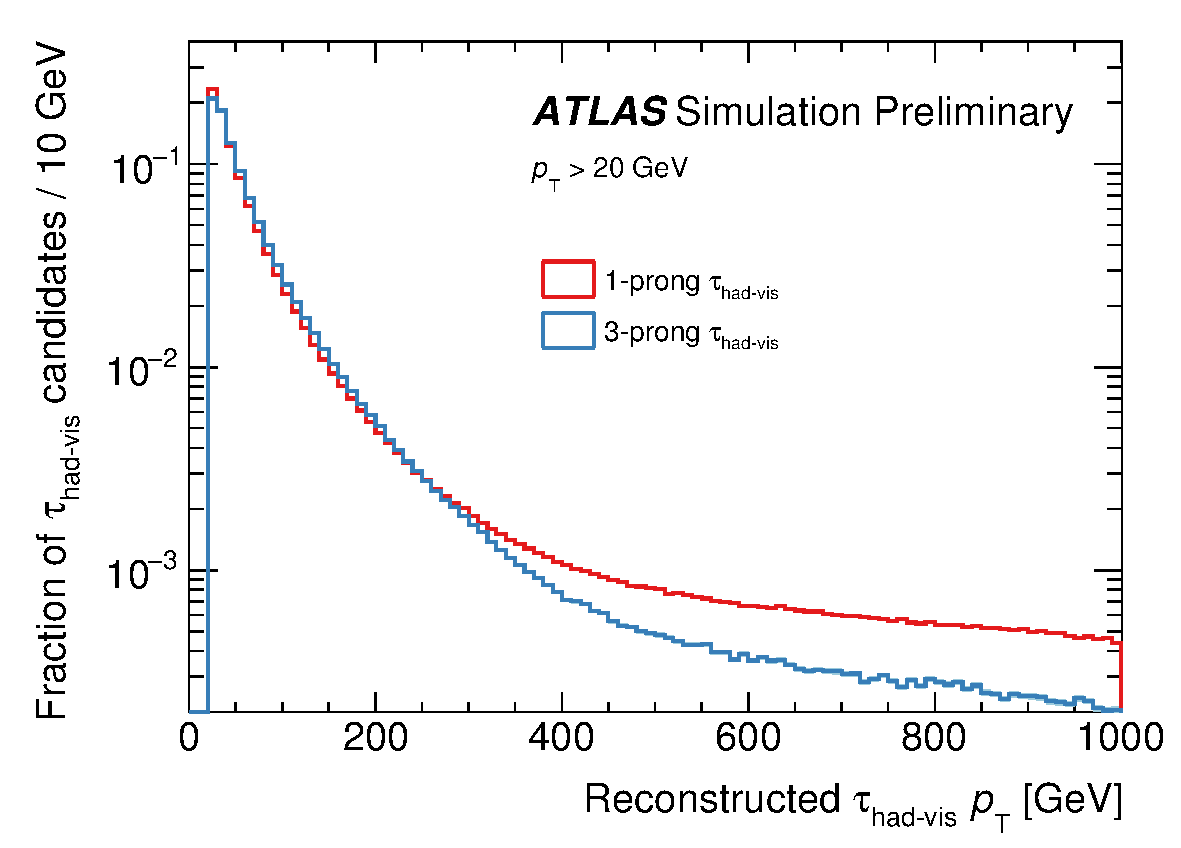
\includegraphics[width=\textwidth]{tauid/pubnote/taupt_gammastar}
    \subcaption{True-\tauhadvis from $\gammastar \to \tautau$ events}%
    \label{fig:tauid_candidate_pt_gammastar}
  \end{subfigure}\hfill%
  \begin{subfigure}{0.498\textwidth}
    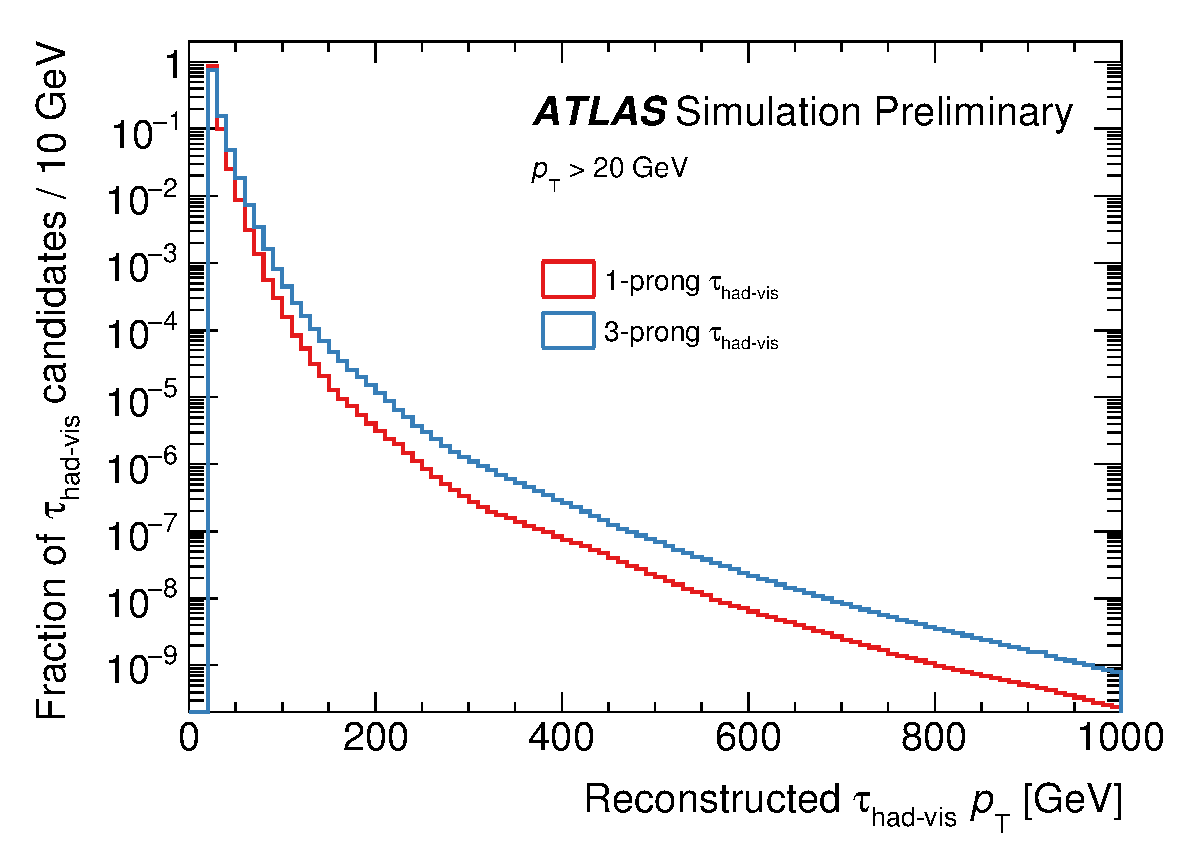
\includegraphics[width=\textwidth]{tauid/pubnote/taupt_dijet}
    \subcaption{Fake-\tauhadvis from di-jet events}%
    \label{fig:tauid_candidate_pt_dijet}
  \end{subfigure}

  \caption{Transverse momentum of 1- and 3-prong \tauhadvis candidates
    in $\gammastar \to \tautau$ (a) and di-jet events (b). Statistical
    uncertainties are shown as coloured bands surrounding the central
    value. Figures taken from Ref.~\cite{ATL-PHYS-PUB-2019-033}.}%
  \label{fig:tauid_candidate_pt}
\end{figure}


\section{Tau Identification with Recurrent Neural Networks}%
\label{sec:tauid_rnn}

The RNN \tauid exploits the discrimination power of both high- and
low-level inputs to distinguish \tauhad from quark- or gluon-initiated
jets. This approach avoids a possible loss of information relevant to
\tauid when manually constructing high-level variables from low-level
inputs. Specifically, charged-particle tracks and clusters of energy
in the calorimeters, hereafter abbreviated as tracks and clusters, are
included as low-level inputs to the algorithm. The inclusion of tracks
and clusters targets the differences in charged and neutral particle
multiplicities and track- and calorimeter-based isolation between
true- and \faketauhadvis.

Tau identification is performed separately for 1- and 3-prong
\tauhadvis candidates due to their distinct signatures.

- Indiciations of large rejection power from track information (while
the information of tracks classified as ``isolation'' are used) ->
More reliant on track classification performance

- How are tracks / clusters associated? How many are used? How are they ordered?


\subsection{Input Variables}

High-level variables

\Cref{fig:tauid_high_level_vars}


\begin{figure}[htbp]
  \centering

  \begin{subfigure}{0.48\textwidth}
    \centering

    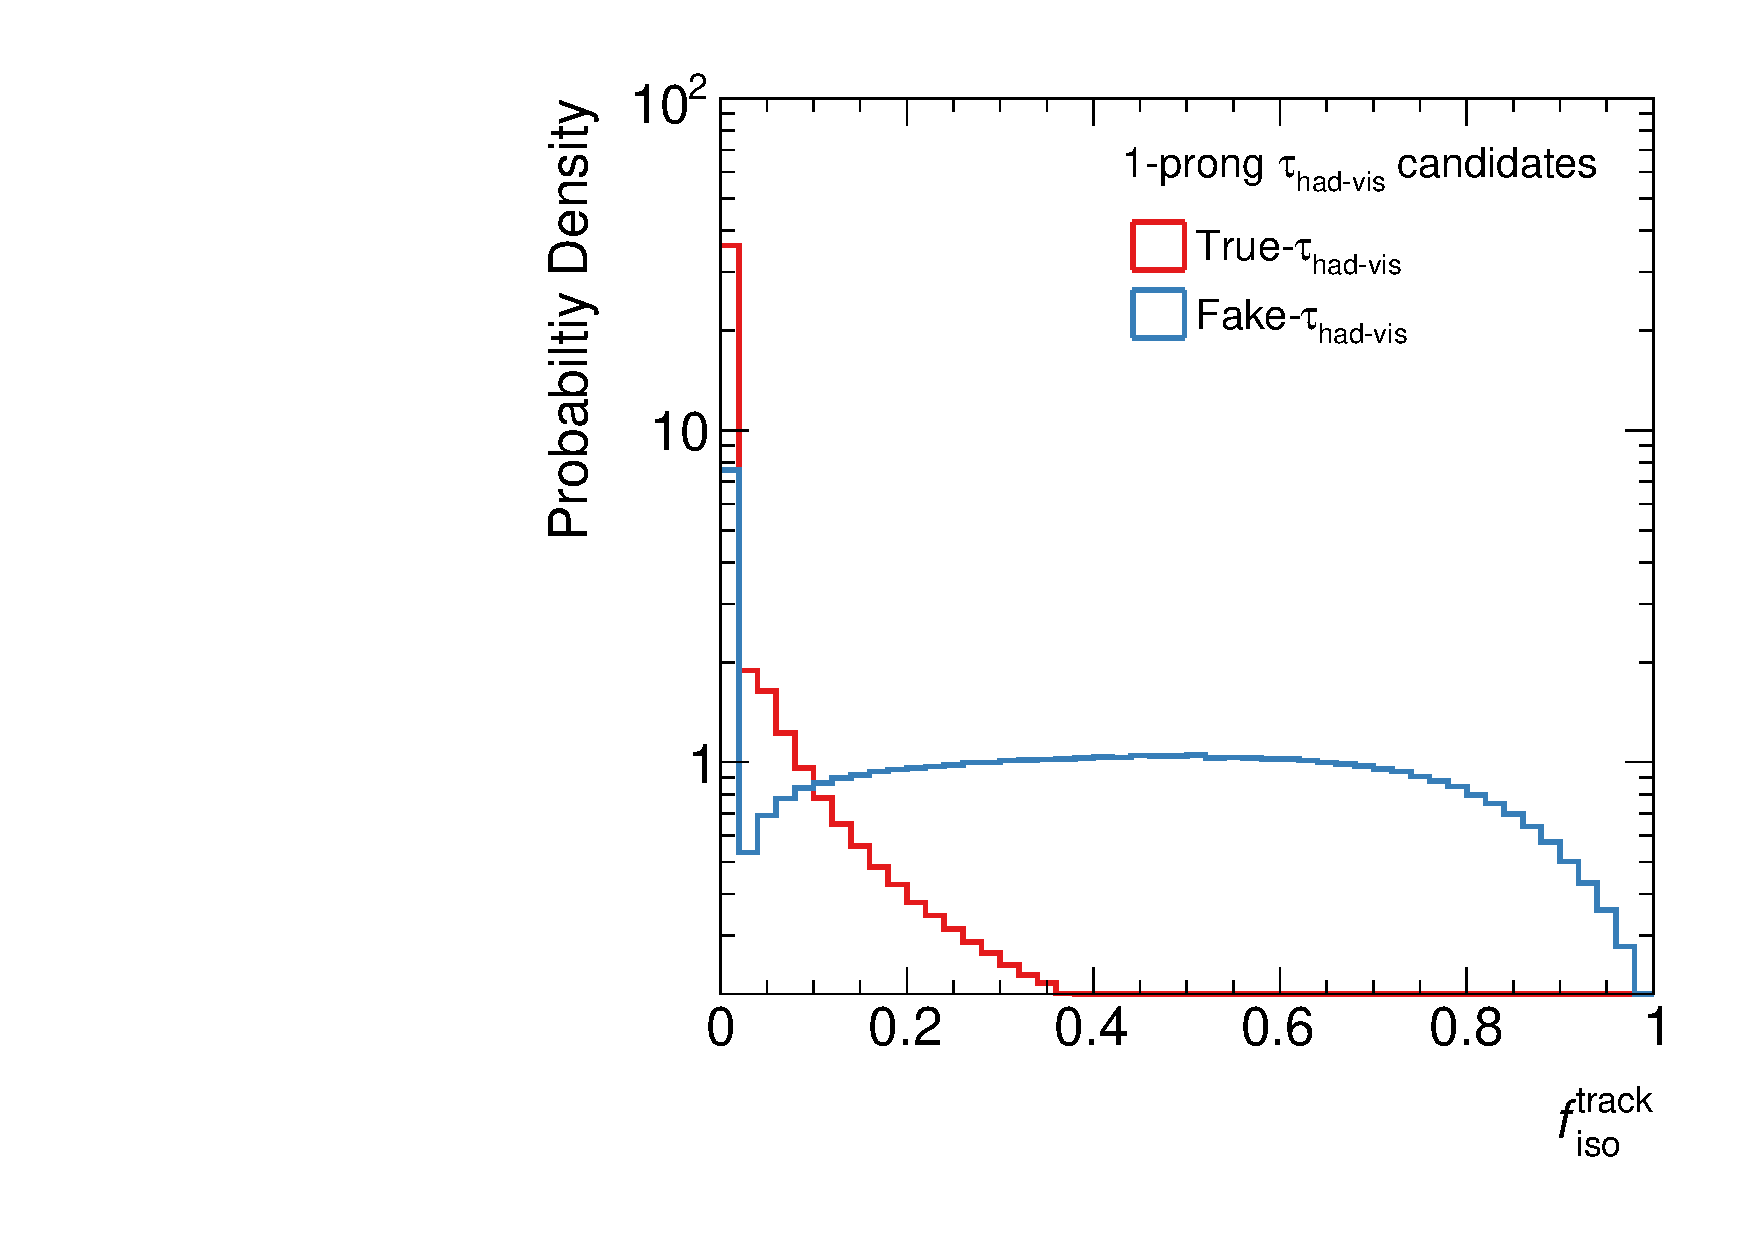
\includegraphics[width=0.67\textwidth]{tauid/invars/invars_sumpttrkfrac_1P}
    \subcaption{}
  \end{subfigure}%
  \begin{subfigure}{0.48\textwidth}
    \centering

    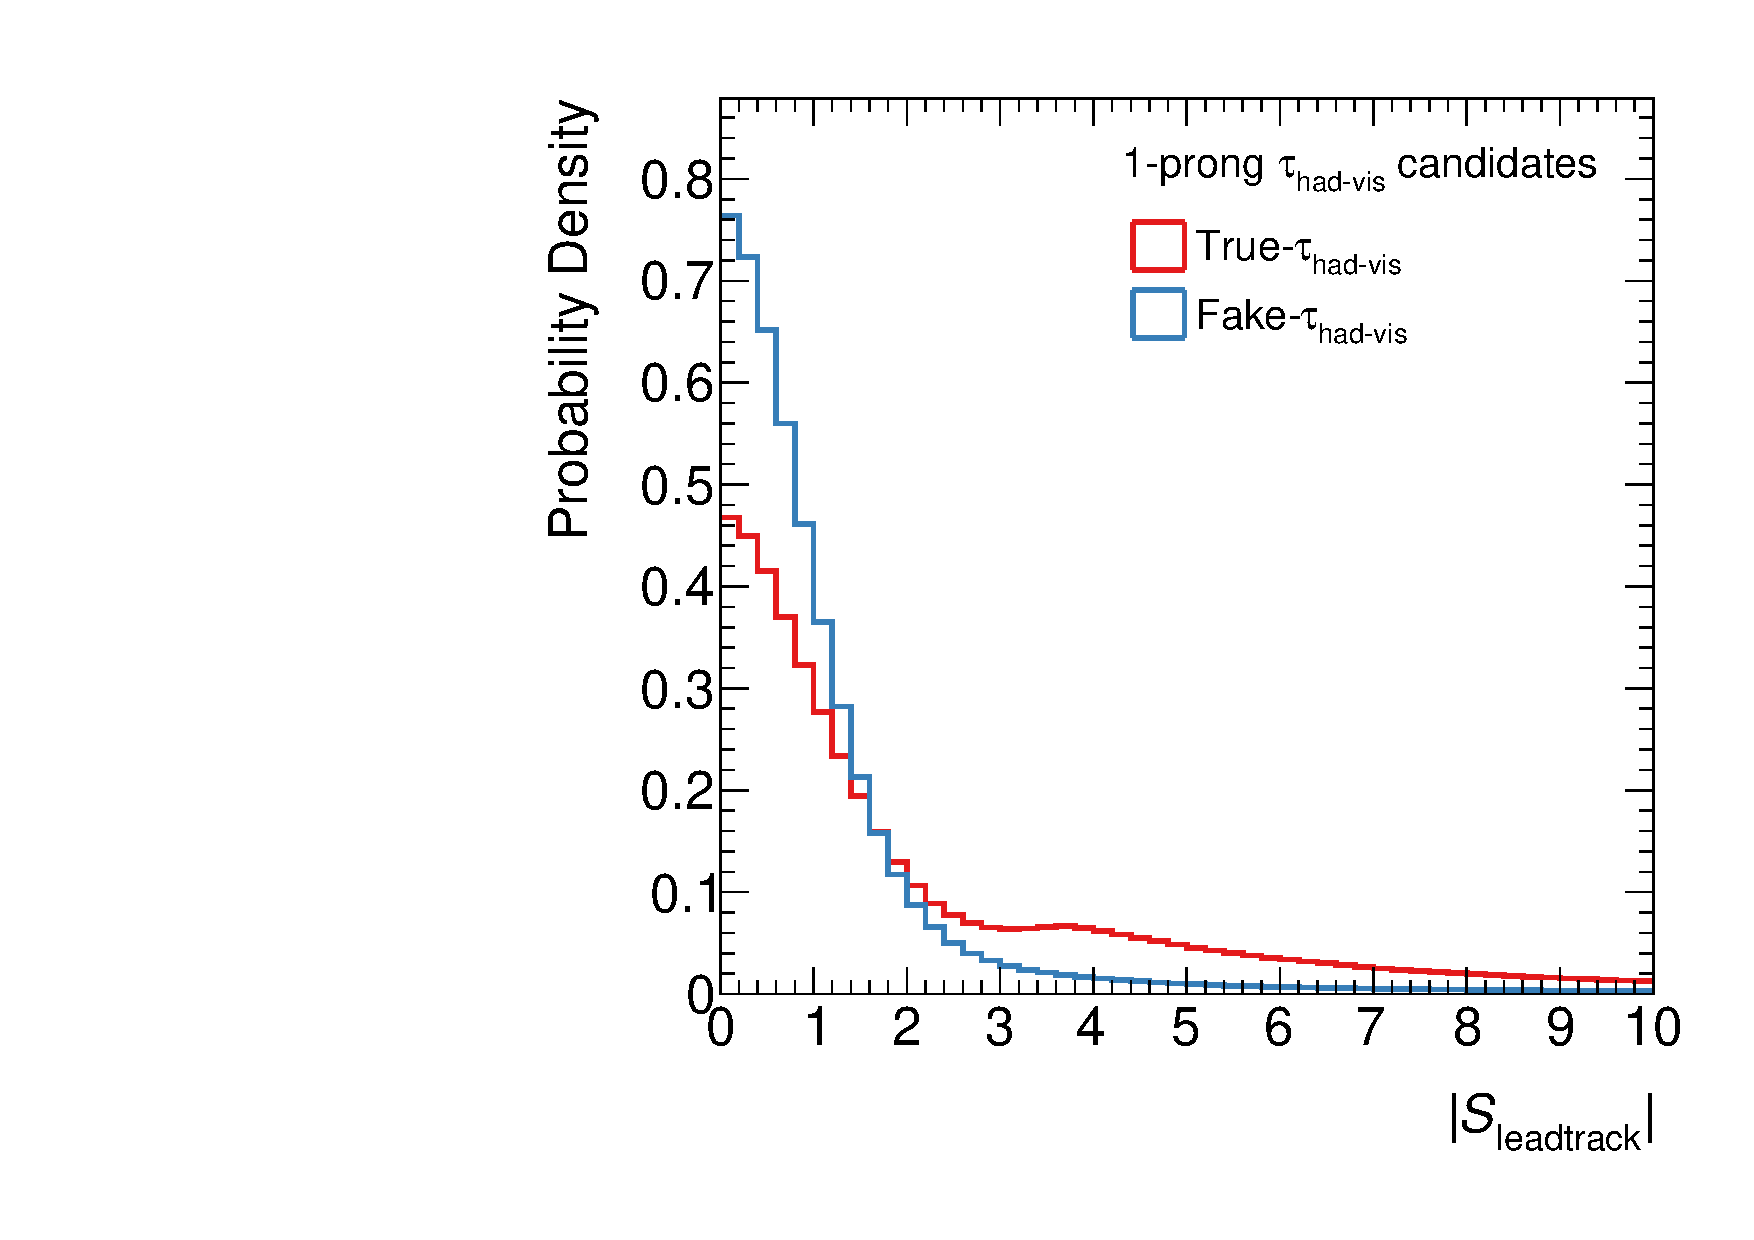
\includegraphics[width=0.67\textwidth]{tauid/invars/invars_absipsigleadtrk_1P}
    \subcaption{}
  \end{subfigure}

  \begin{subfigure}{0.48\textwidth}
    \centering

    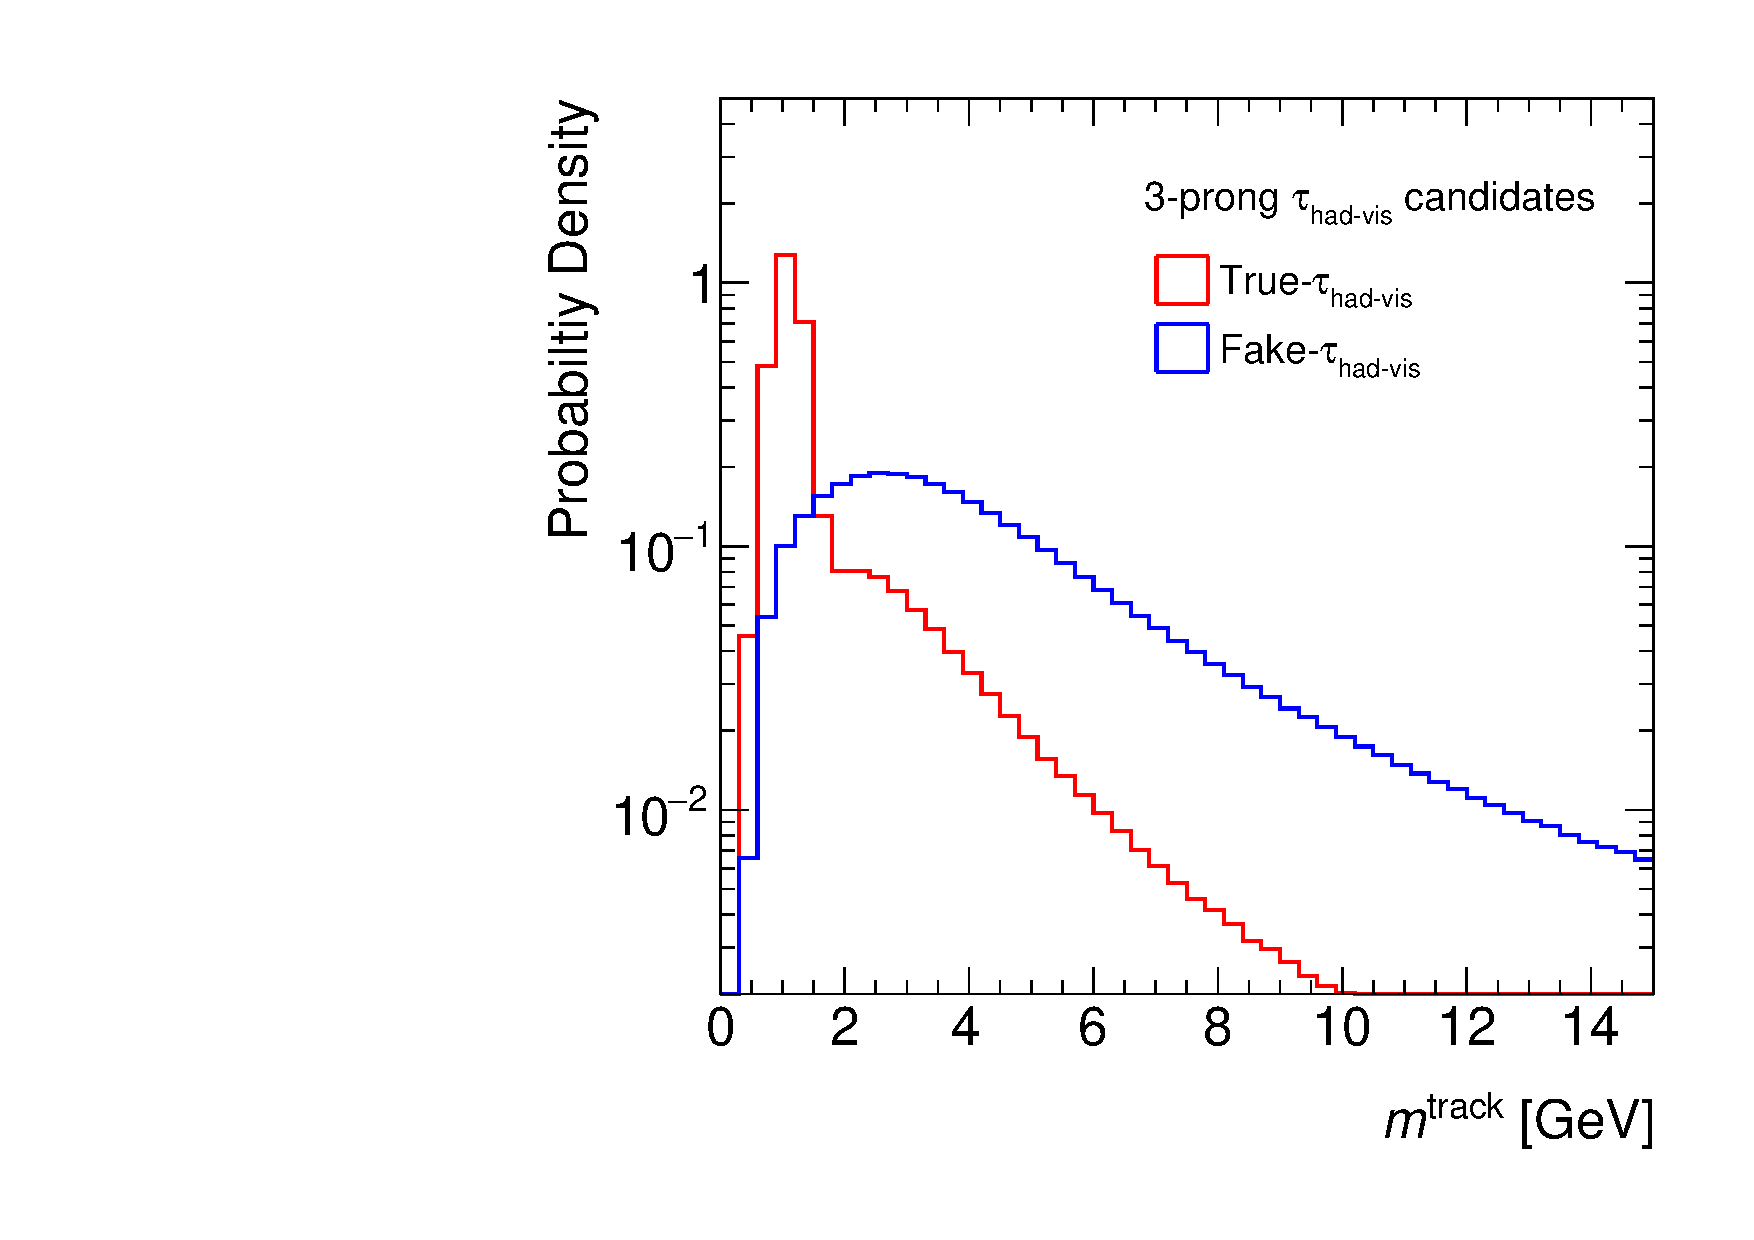
\includegraphics[width=0.67\textwidth]{tauid/invars/invars_masstrksys_3P}
    \subcaption{}
  \end{subfigure}%
  \begin{subfigure}{0.48\textwidth}
    \centering

    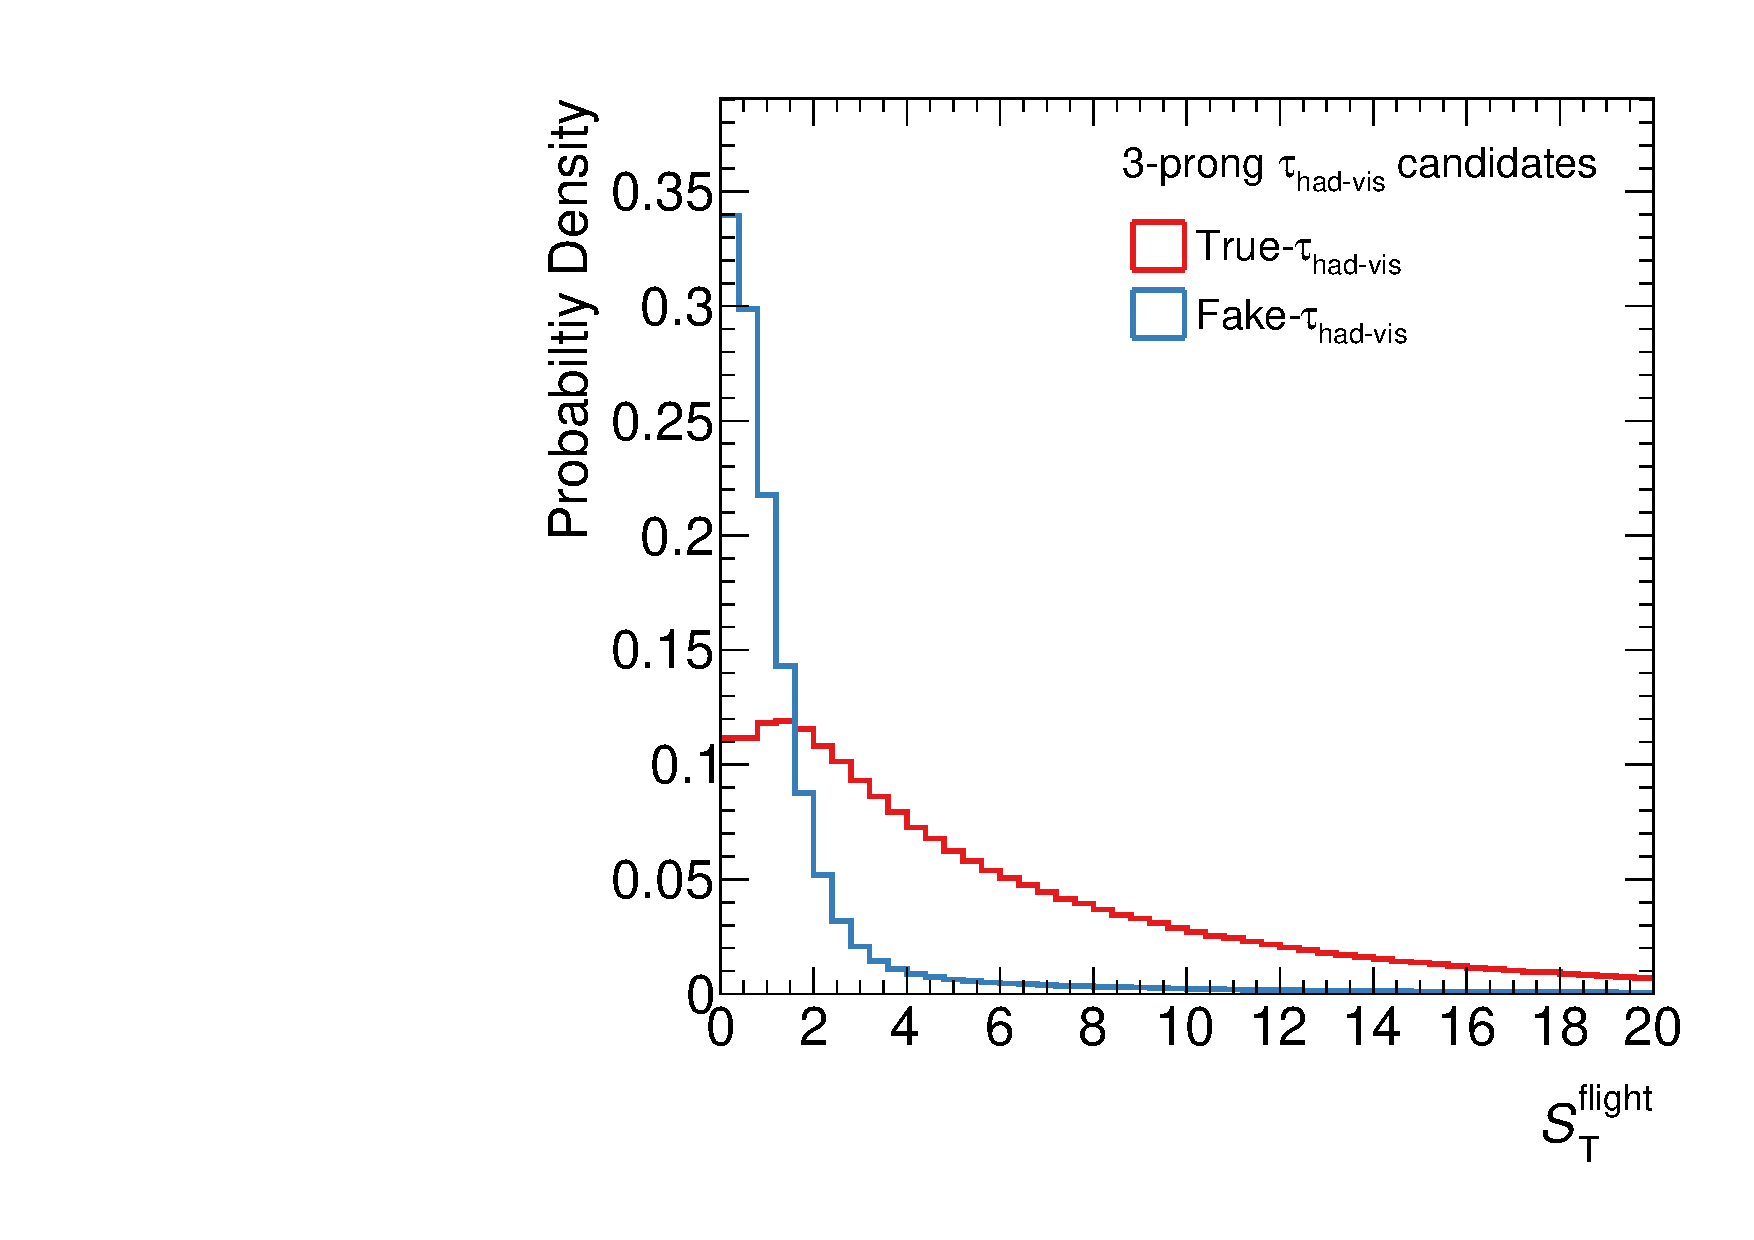
\includegraphics[width=0.67\textwidth]{tauid/invars/invars_trflightpathsig_3P}
    \subcaption{}
  \end{subfigure}

  \caption{Selected high-level input variables}%
  \label{fig:tauid_high_level_vars}
\end{figure}


Tracks: How associated.

All reconstructed tracks within $\Delta R < 0.4$ of the \tauhadvis
candidate axis with $\pT > \SI{500}{\MeV}$ are considered as inputs to
the to the RNN \tauid. The tracks associated to \tauhadvis candidates
include fake tracks and pile-up tracks. Have to include impact
parameters and track quality criteria.


\begin{figure}[htbp]
  \centering

  \begin{subfigure}{0.33\textwidth}
    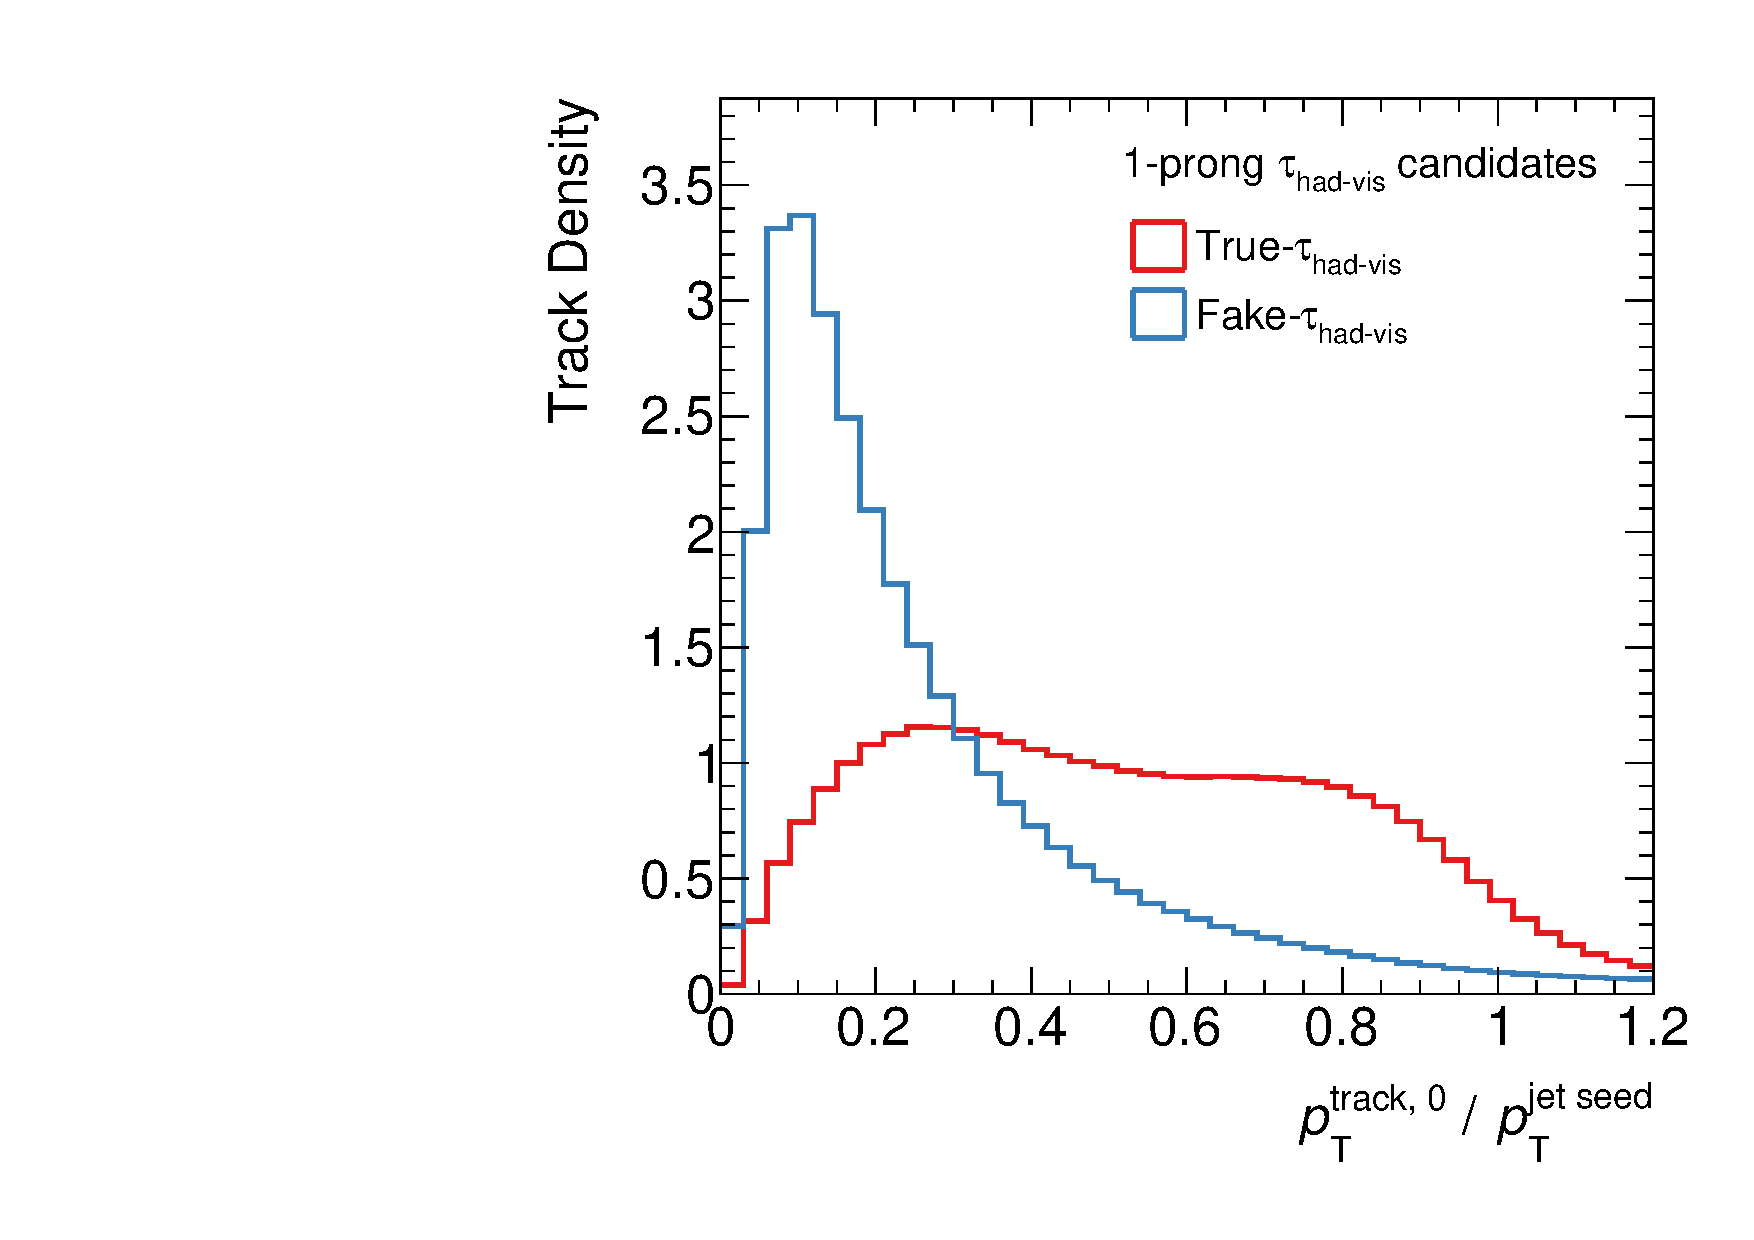
\includegraphics[width=\textwidth]{tauid/invars/invars_trk0relpt_1P}
    \subcaption{}
  \end{subfigure}%
  \begin{subfigure}{0.33\textwidth}
    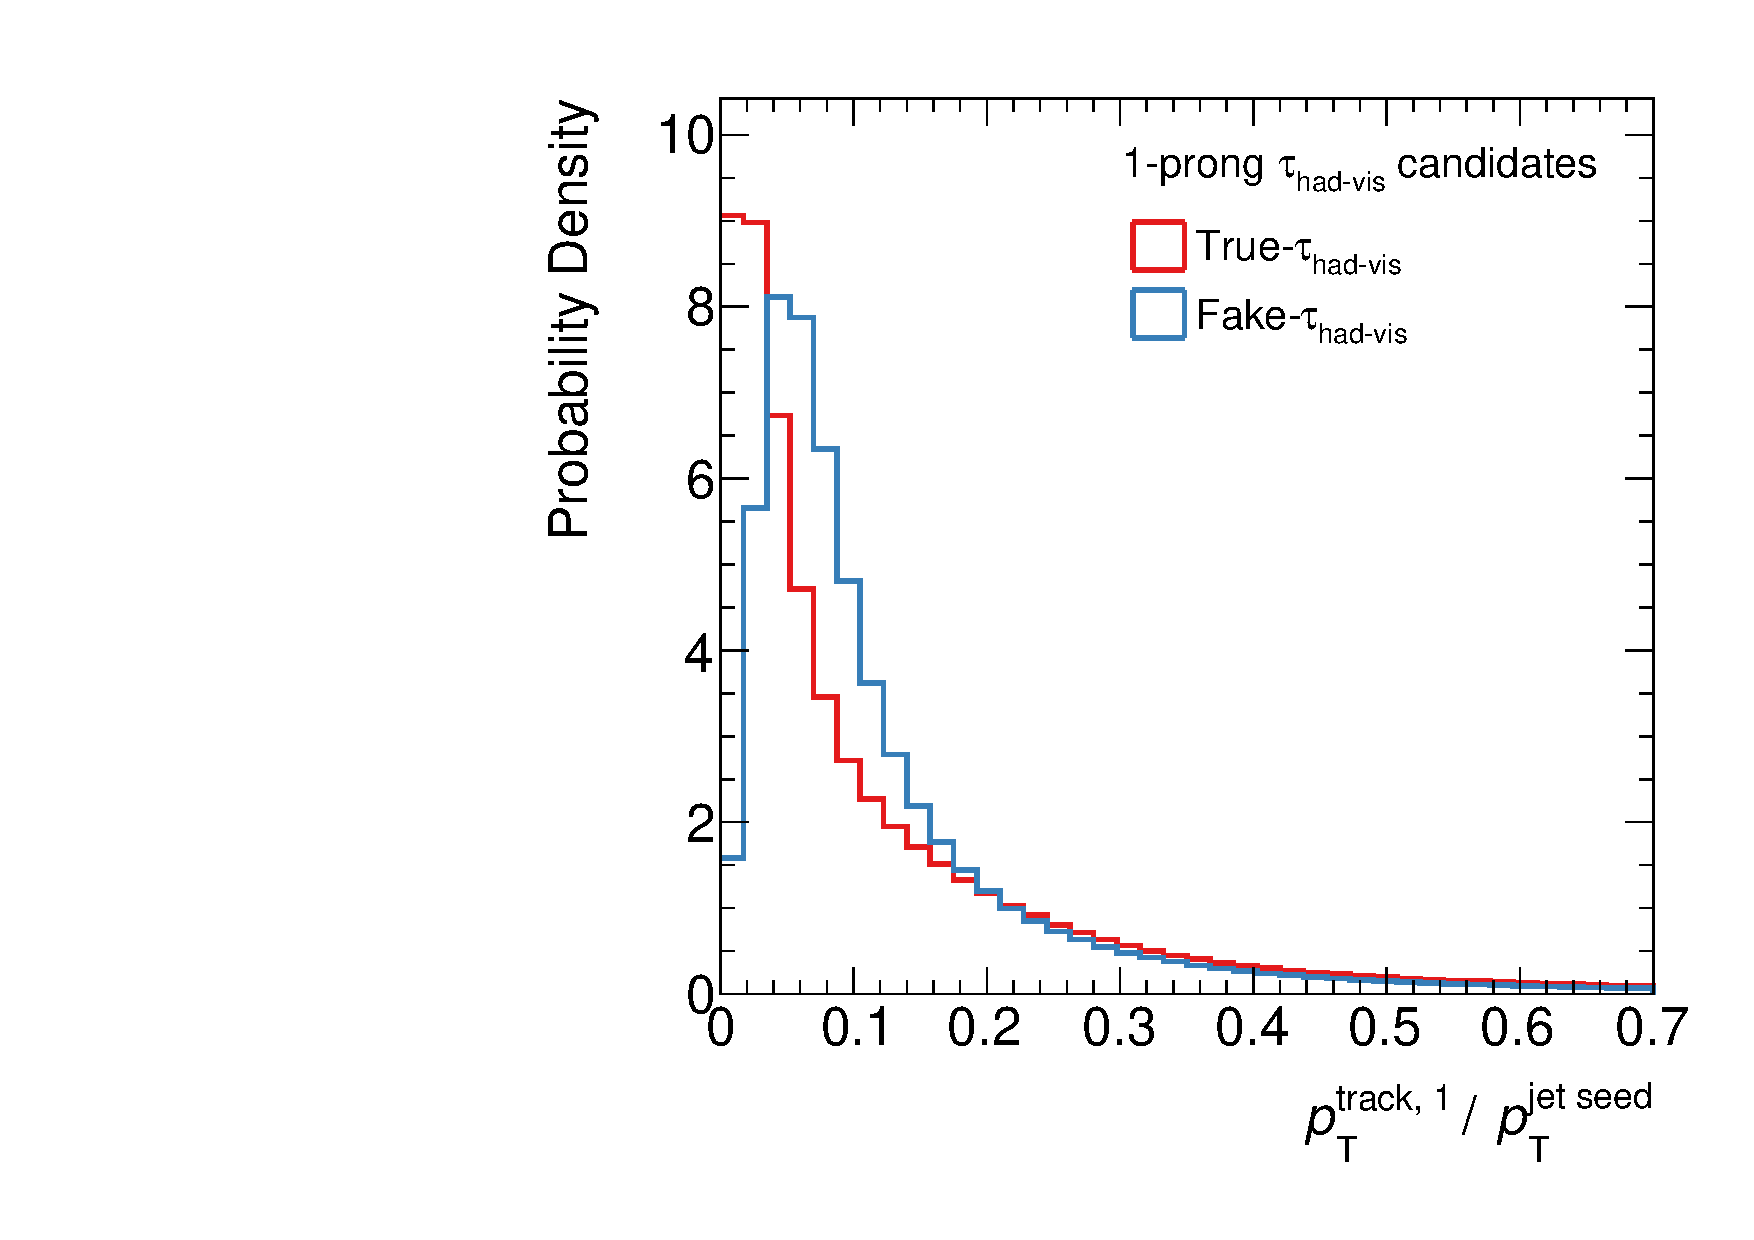
\includegraphics[width=\textwidth]{tauid/invars/invars_trk1relpt_1P}
    \subcaption{}
  \end{subfigure}%
  \begin{subfigure}{0.33\textwidth}
    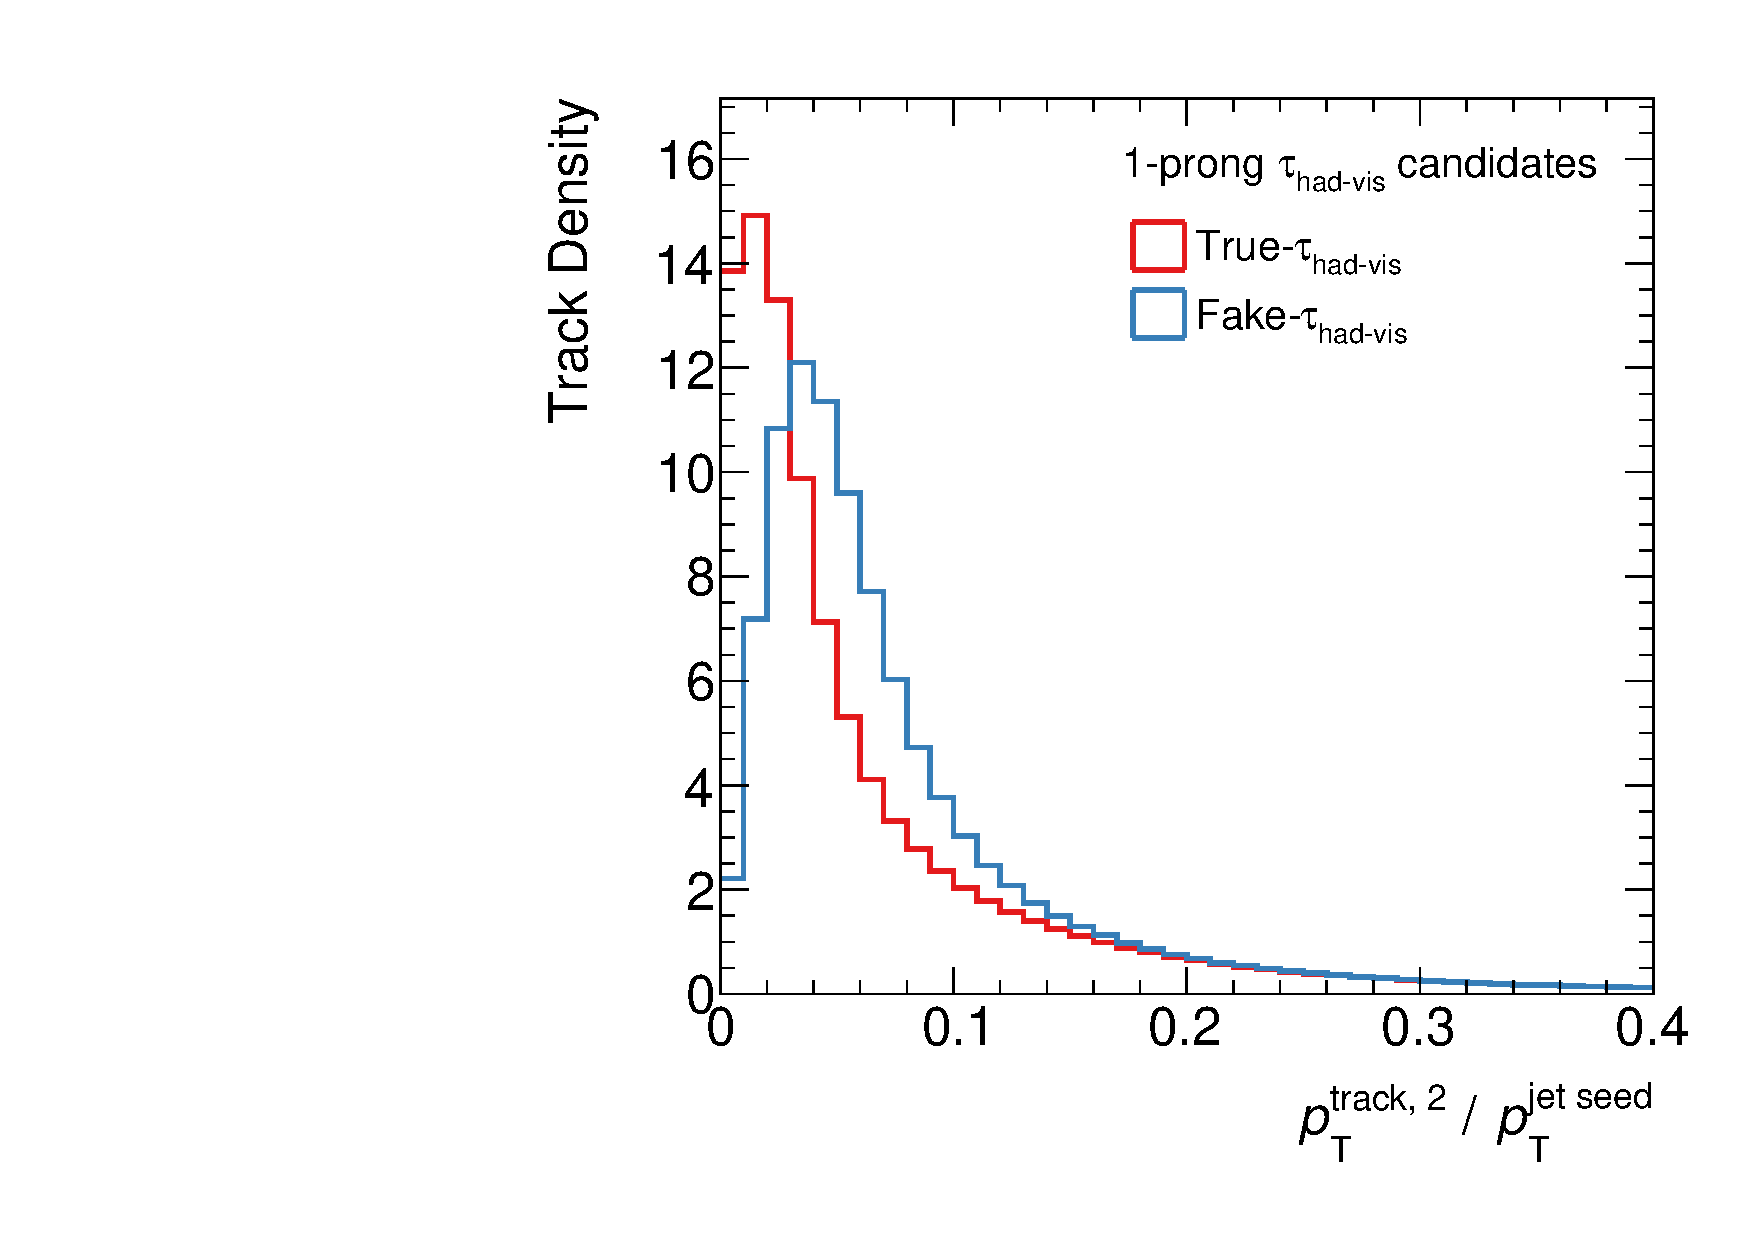
\includegraphics[width=\textwidth]{tauid/invars/invars_trk2relpt_1P}
    \subcaption{}
  \end{subfigure}

  \begin{subfigure}{0.33\textwidth}
    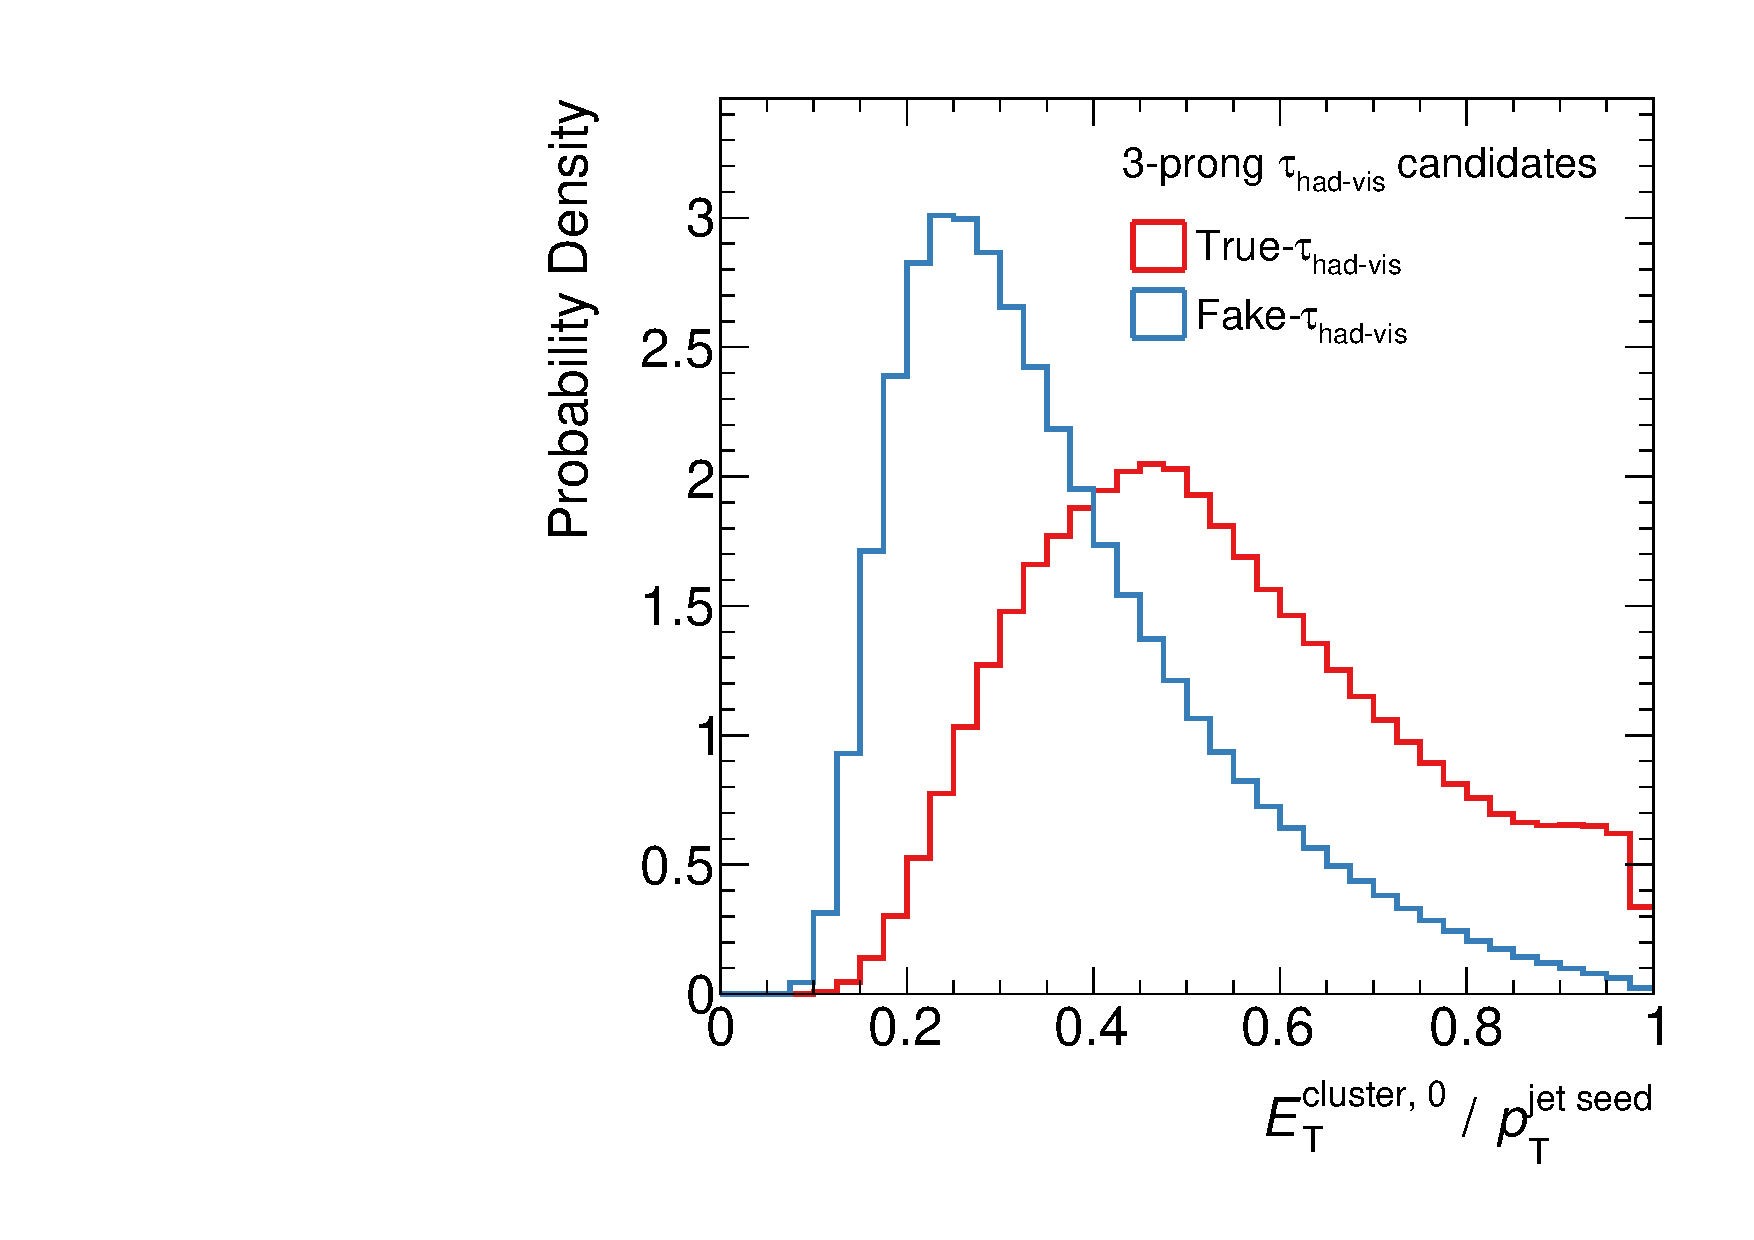
\includegraphics[width=\textwidth]{tauid/invars/invars_cls0relet_3P}
    \subcaption{}
  \end{subfigure}%
  \begin{subfigure}{0.33\textwidth}
    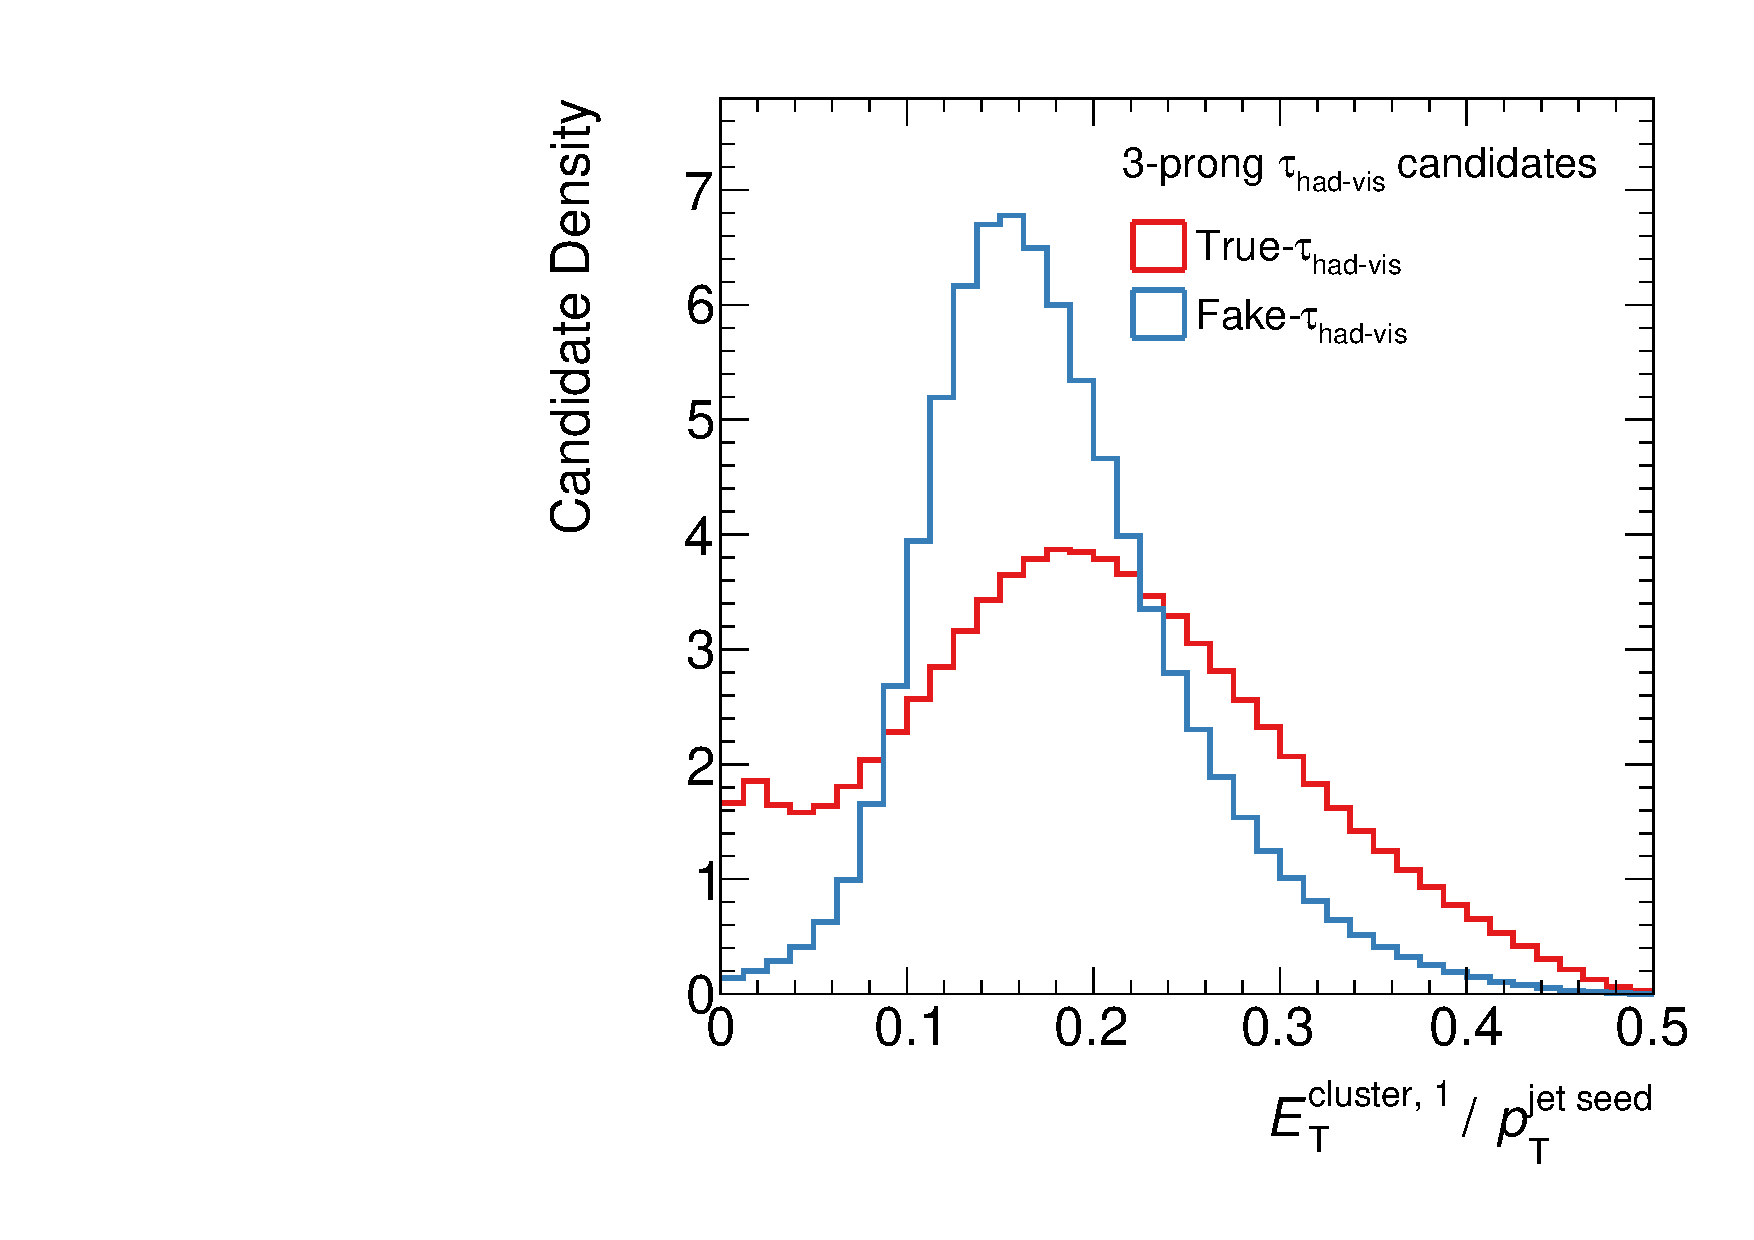
\includegraphics[width=\textwidth]{tauid/invars/invars_cls1relet_3P}
    \subcaption{}
  \end{subfigure}%
  \begin{subfigure}{0.33\textwidth}
    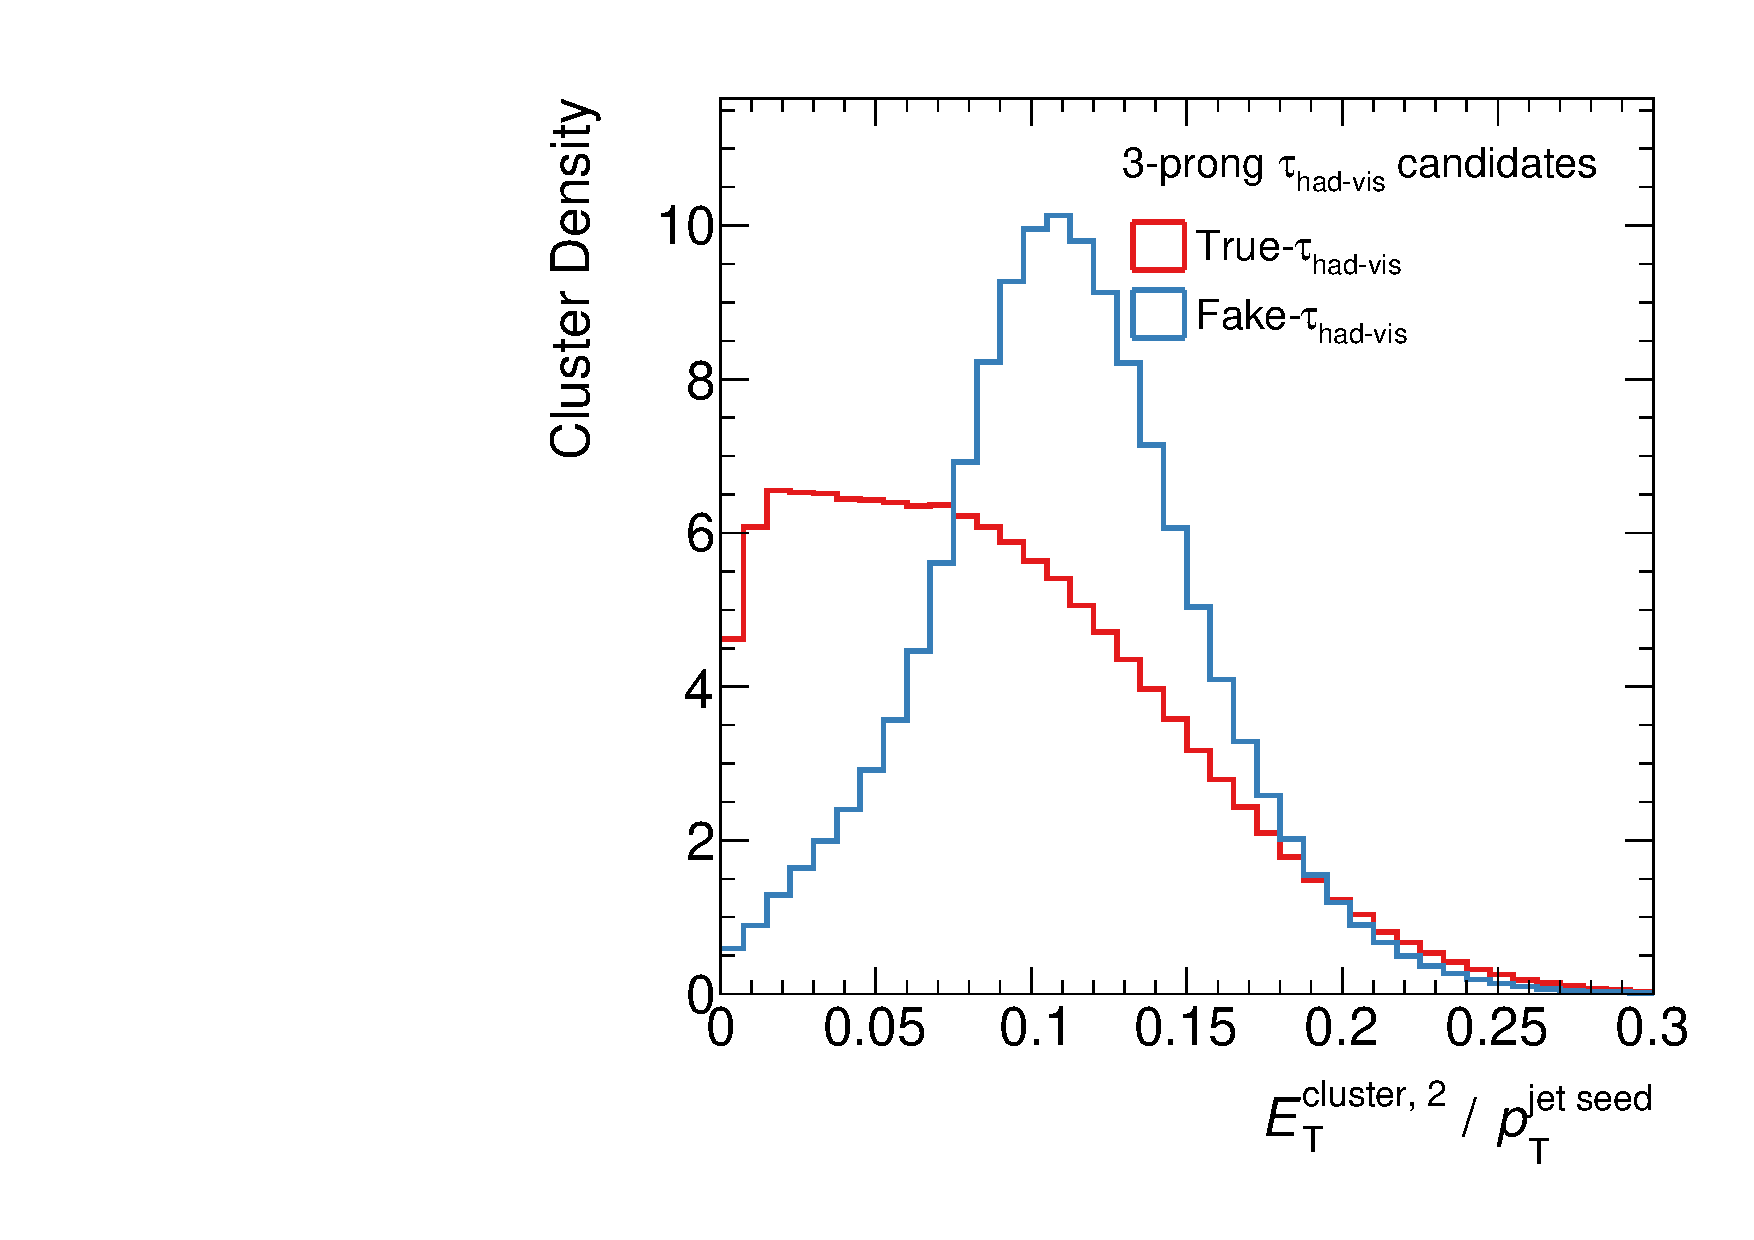
\includegraphics[width=\textwidth]{tauid/invars/invars_cls2relet_3P}
    \subcaption{}
  \end{subfigure}

  \caption{Sequence variables}%
  \label{fig:tauid_low_level_variables}
\end{figure}


% \begin{figure}[htbp]
%   \centering

%   \begin{subfigure}{0.33\textwidth}
%     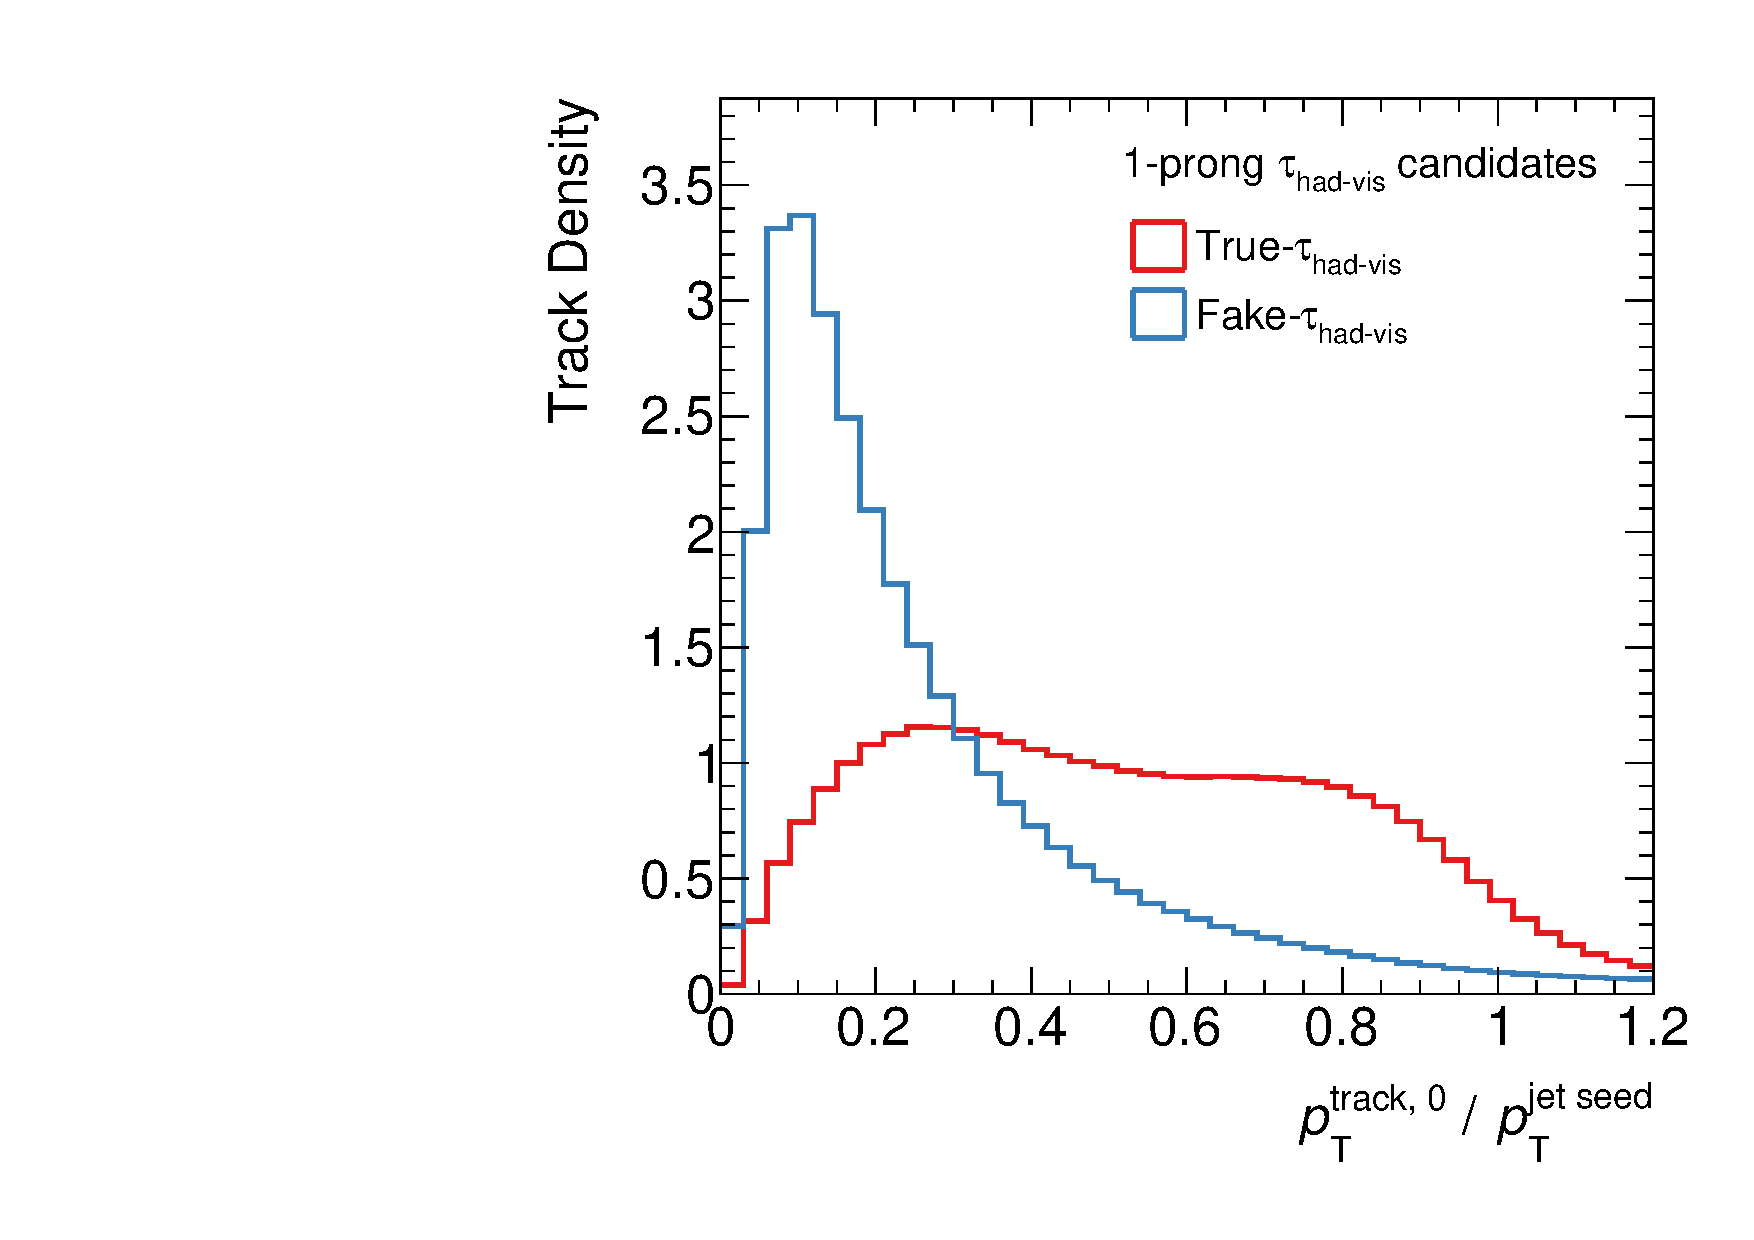
\includegraphics[width=\textwidth]{tauid/invars/invars_trk0relpt_1P}
%     \subcaption{}
%   \end{subfigure}%
%   \begin{subfigure}{0.33\textwidth}
%     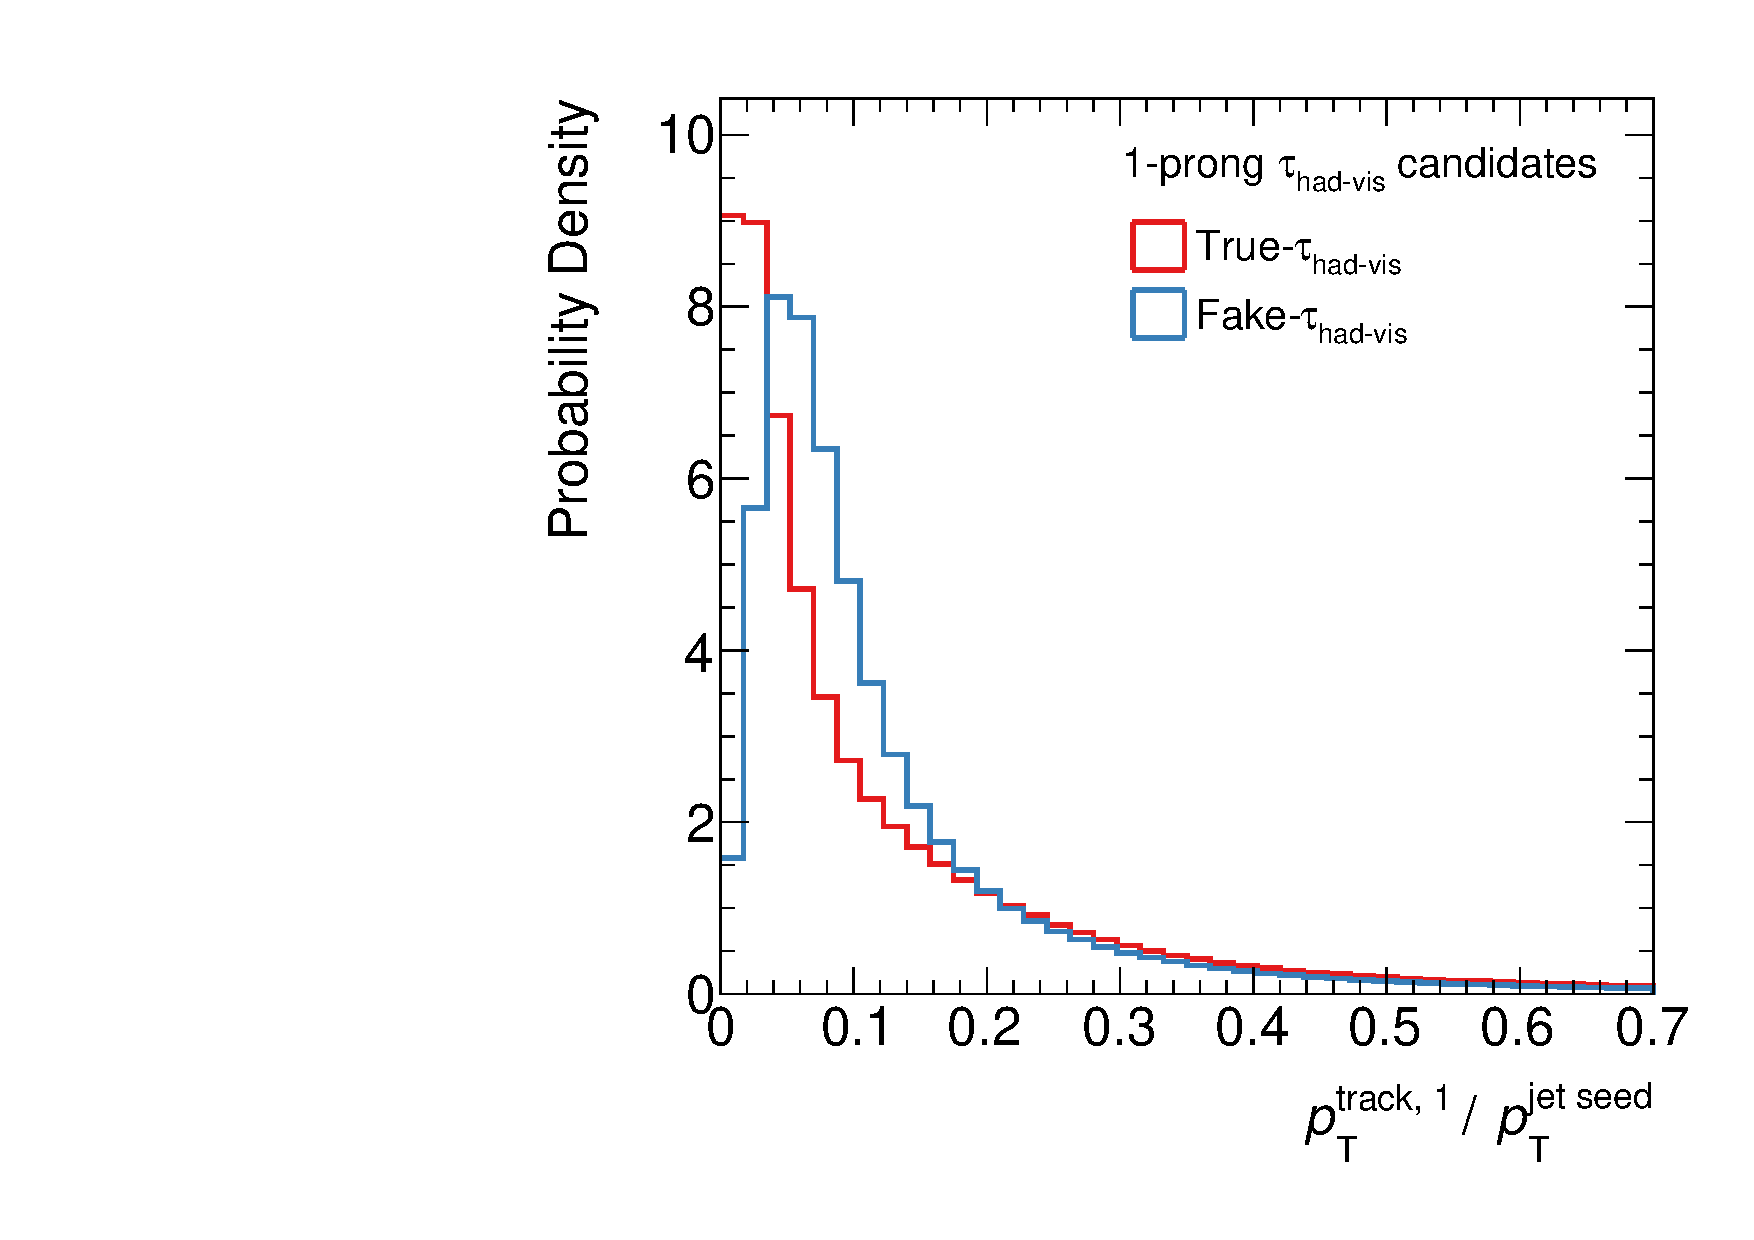
\includegraphics[width=\textwidth]{tauid/invars/invars_trk1relpt_1P}
%     \subcaption{}
%   \end{subfigure}%
%   \begin{subfigure}{0.33\textwidth}
%     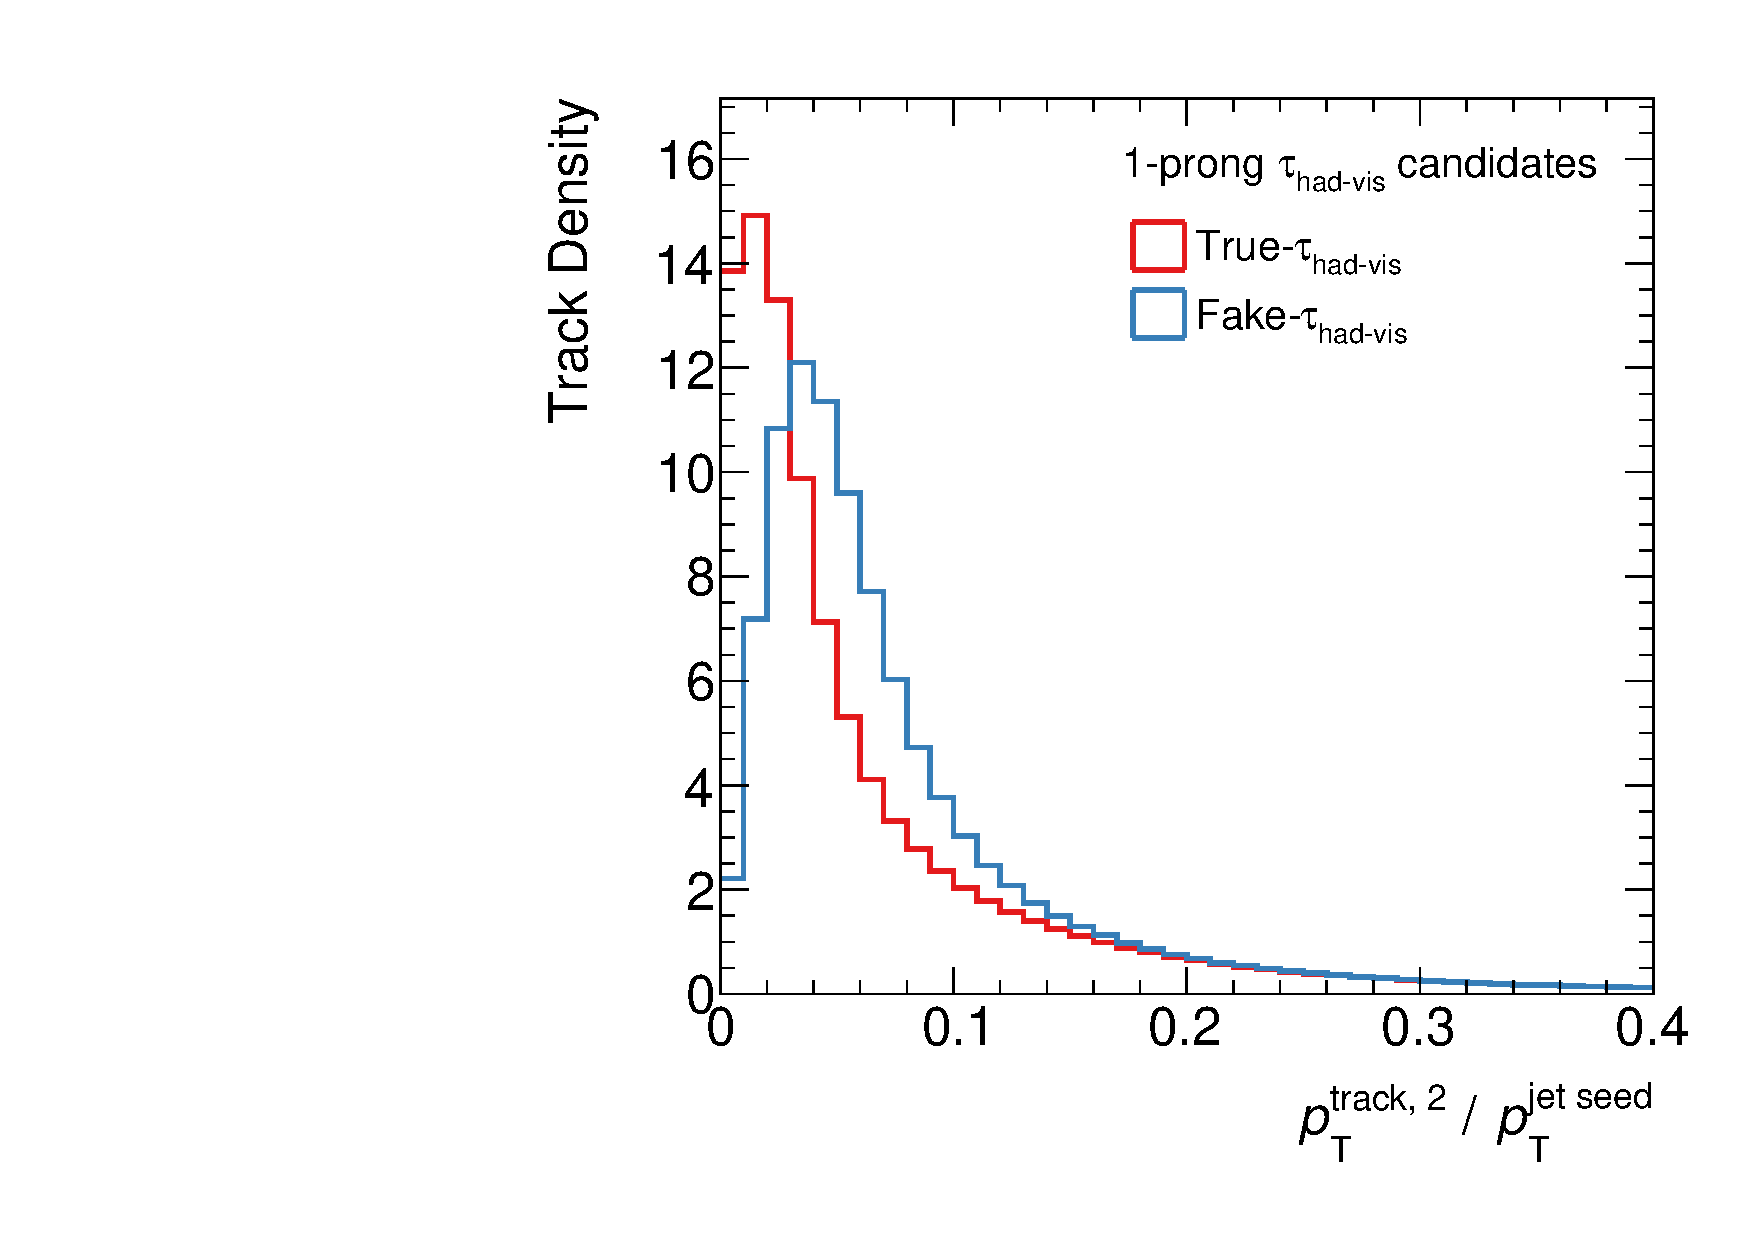
\includegraphics[width=\textwidth]{tauid/invars/invars_trk2relpt_1P}
%     \subcaption{}
%   \end{subfigure}

%   \begin{subfigure}{0.33\textwidth}
%     \includegraphics[width=\textwidth]{tauid/invars/invars_trk0relpt_3P}
%     \subcaption{}
%   \end{subfigure}%
%   \begin{subfigure}{0.33\textwidth}
%     \includegraphics[width=\textwidth]{tauid/invars/invars_trk1relpt_3P}
%     \subcaption{}
%   \end{subfigure}%
%   \begin{subfigure}{0.33\textwidth}
%     \includegraphics[width=\textwidth]{tauid/invars/invars_trk2relpt_3P}
%     \subcaption{}
%   \end{subfigure}

%   \caption{Sequence variables}%
%   \label{fig:tauid_low_level_variables}
% \end{figure}

% \begin{figure}[htbp]
%   \centering

%   \begin{subfigure}{0.33\textwidth}
%     \includegraphics[width=\textwidth]{tauid/invars/invars_cls0relet_1P}
%     \subcaption{}
%   \end{subfigure}%
%   \begin{subfigure}{0.33\textwidth}
%     \includegraphics[width=\textwidth]{tauid/invars/invars_cls1relet_1P}
%     \subcaption{}
%   \end{subfigure}%
%   \begin{subfigure}{0.33\textwidth}
%     \includegraphics[width=\textwidth]{tauid/invars/invars_cls2relet_1P}
%     \subcaption{}
%   \end{subfigure}

%   \begin{subfigure}{0.33\textwidth}
%     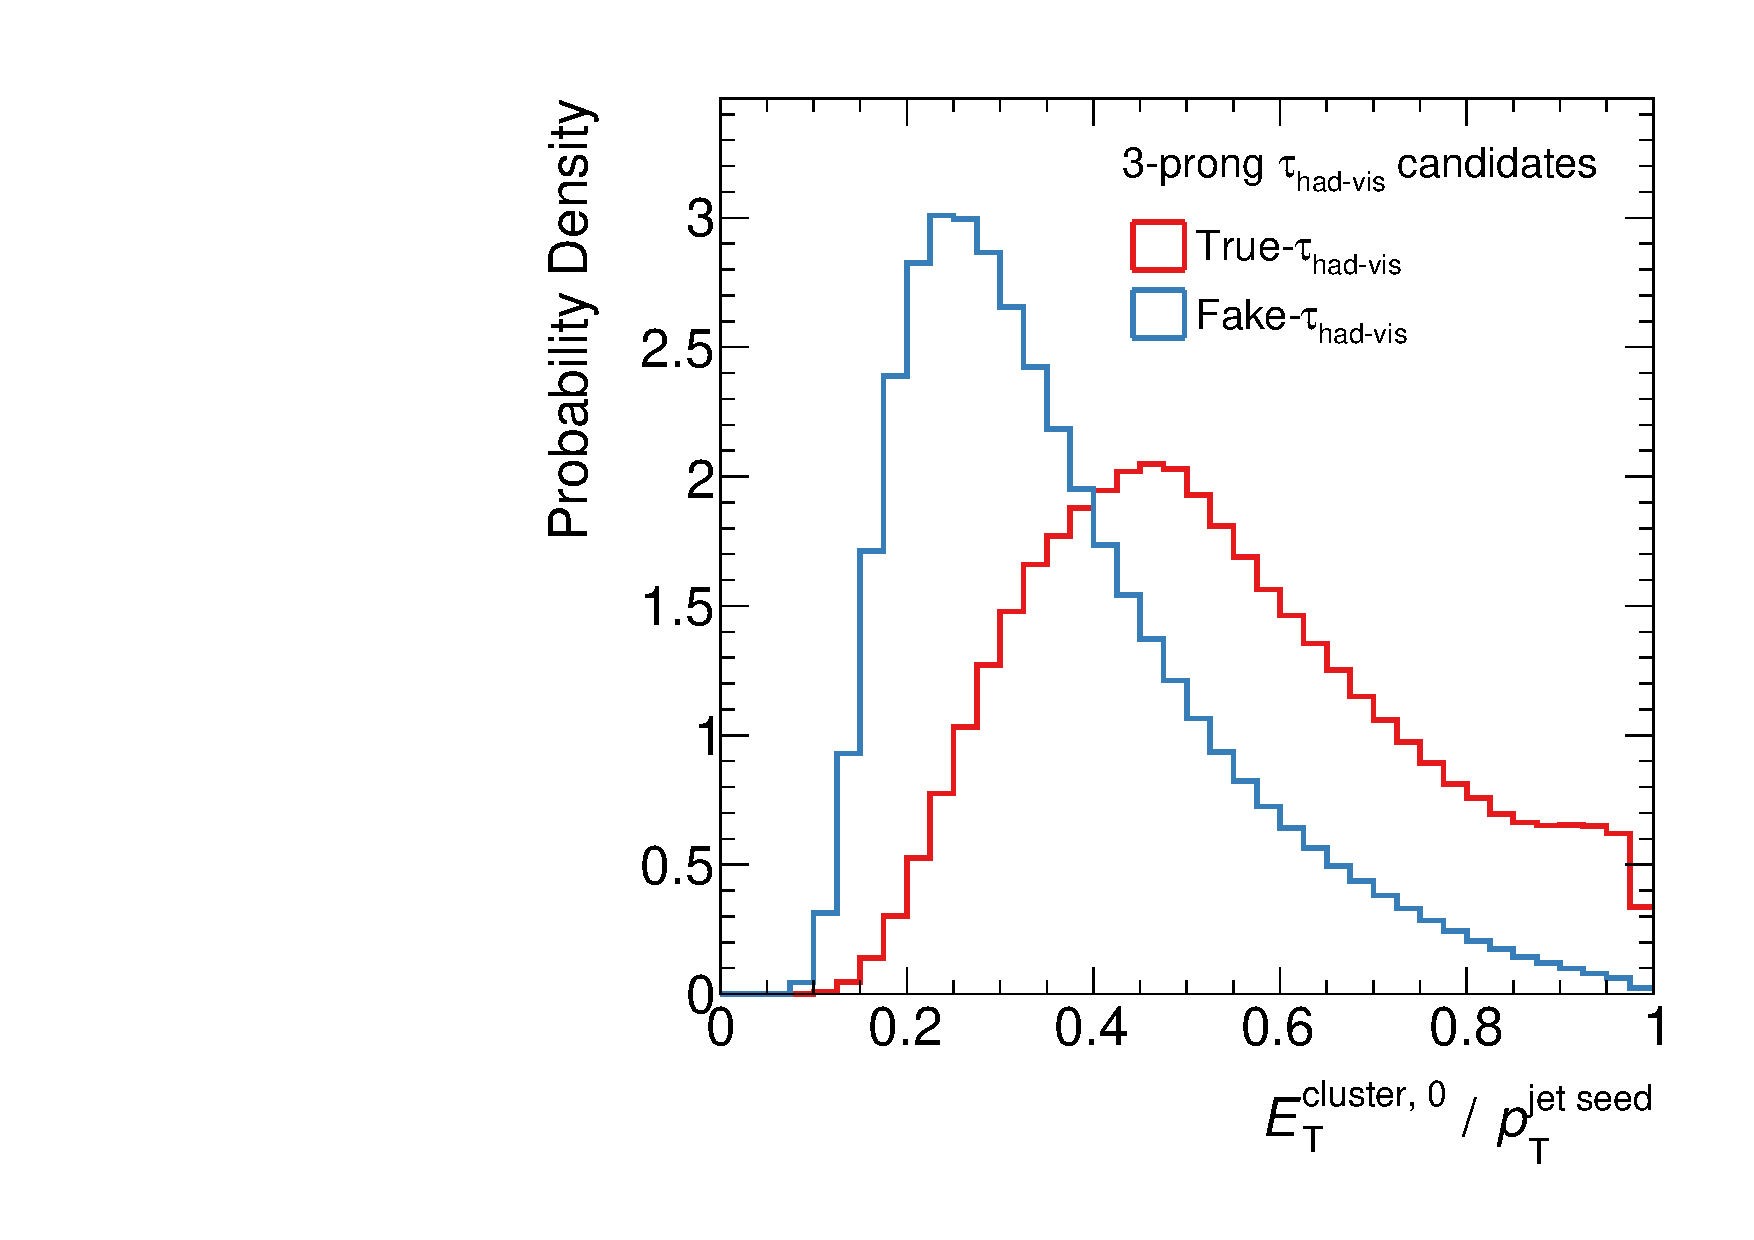
\includegraphics[width=\textwidth]{tauid/invars/invars_cls0relet_3P}
%     \subcaption{}
%   \end{subfigure}%
%   \begin{subfigure}{0.33\textwidth}
%     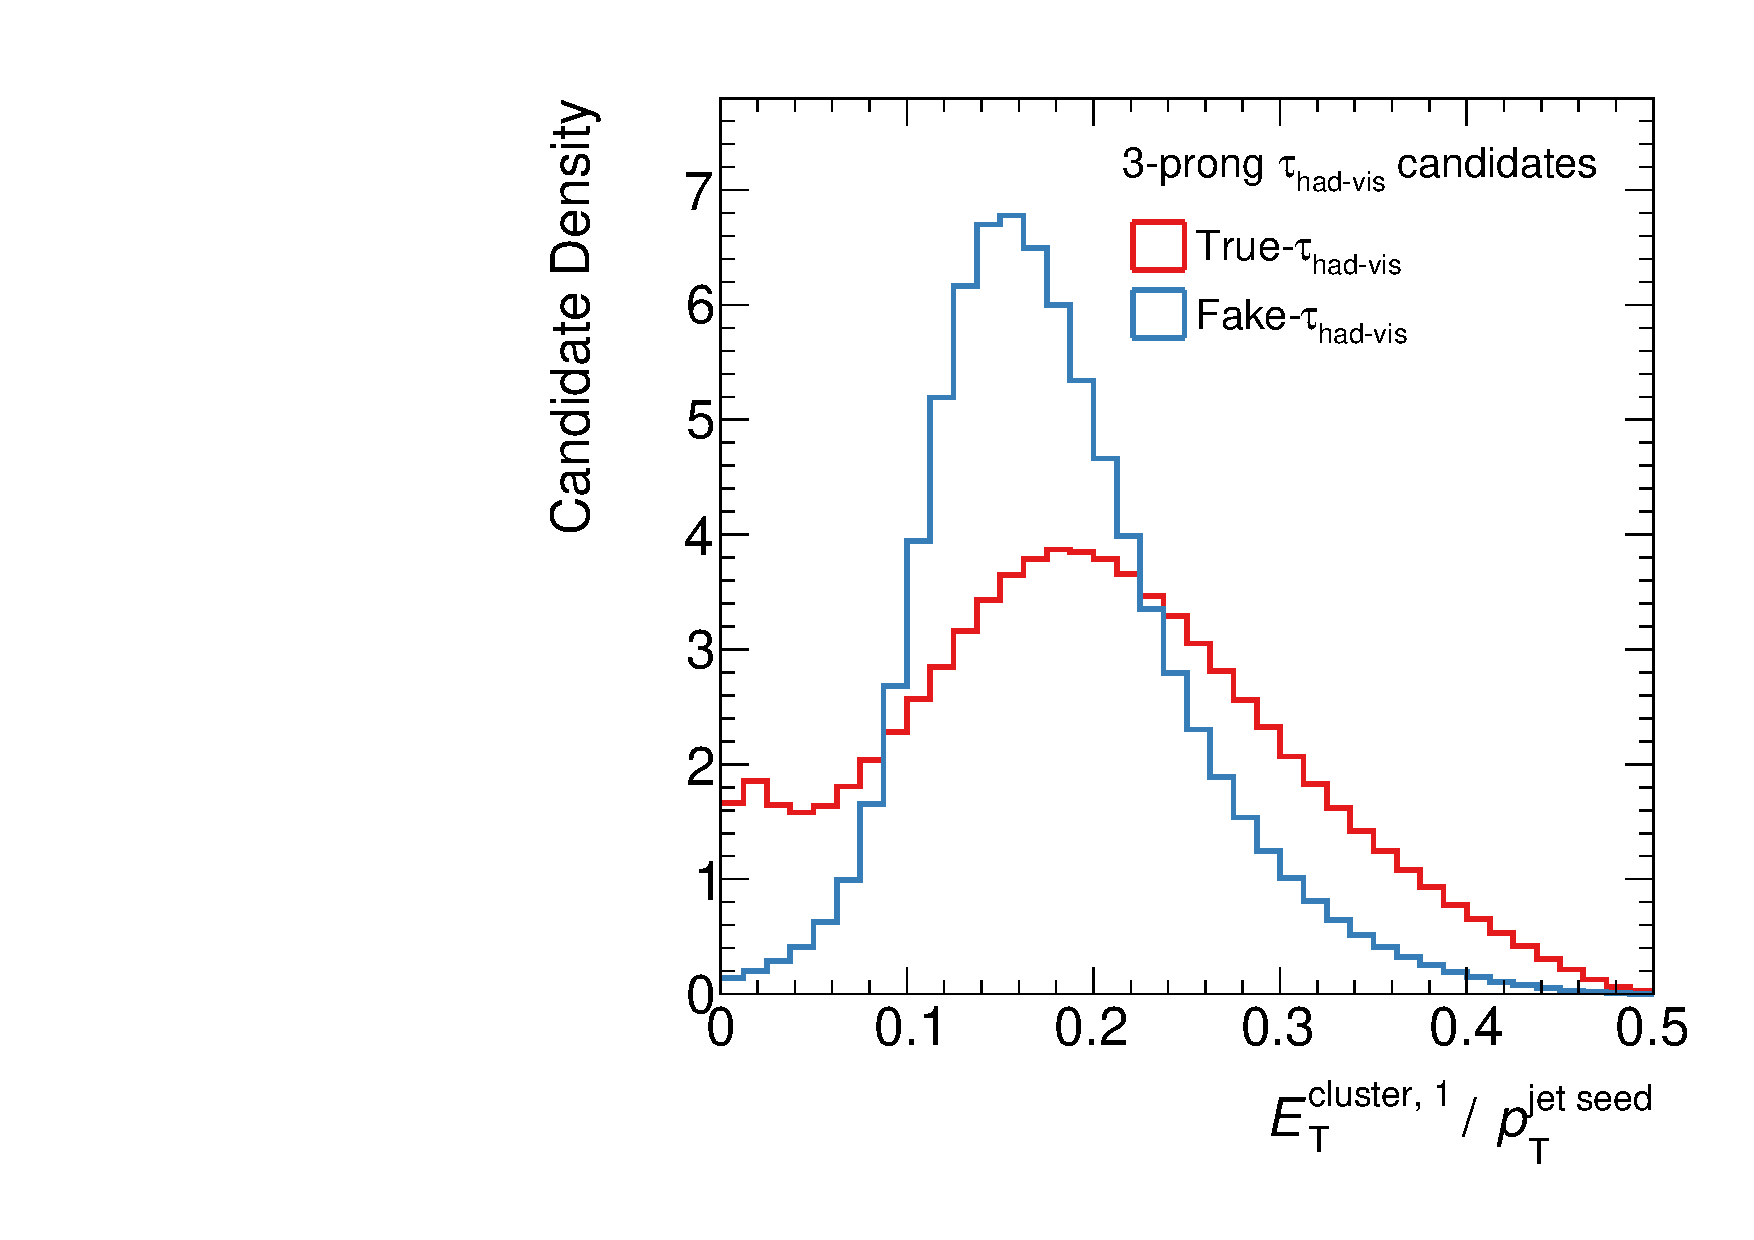
\includegraphics[width=\textwidth]{tauid/invars/invars_cls1relet_3P}
%     \subcaption{}
%   \end{subfigure}%
%   \begin{subfigure}{0.33\textwidth}
%     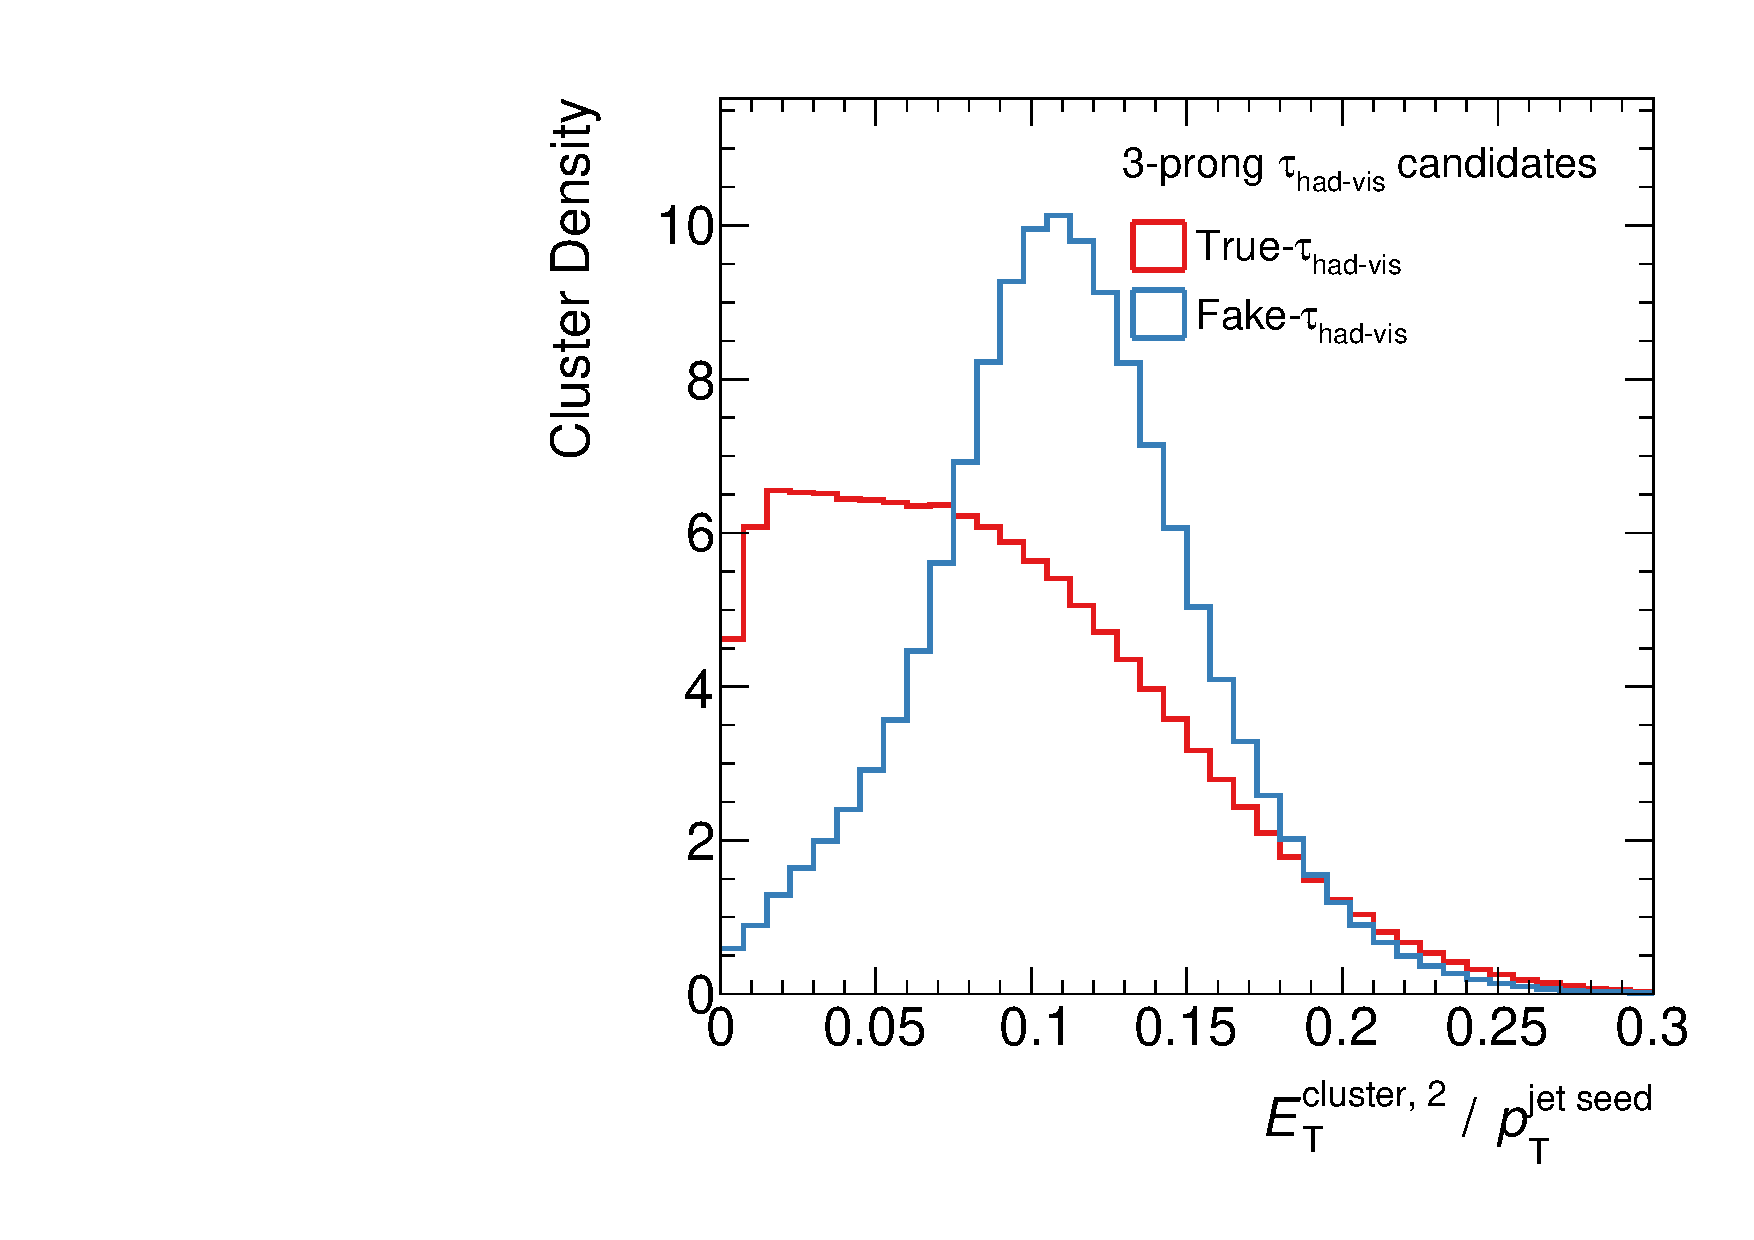
\includegraphics[width=\textwidth]{tauid/invars/invars_cls2relet_3P}
%     \subcaption{}
%   \end{subfigure}

%   \caption{Sequence variables}%
%   \label{fig:tauid_low_level_variables_2}
% \end{figure}


Clusters: How associated.

Clusters are considered if they are
constituents of the jet that seeded the \tauhadvis reconstruction.




\begin{table}[htbp]
  \centering

  \caption{Input variables. Adopted from
    Ref.~\cite{ATL-PHYS-PUB-2019-033}.}%
  \label{tab:tauid_input_variables}

  \renewcommand{\arraystretch}{1.2}

\begin{tabular}{clccp{10.5cm}}
  \toprule
  & Observable & 1-prong & 3-prong & Description \\
  \midrule
  \parbox[t]{2mm}{\multirow{11}{*}{\rotatebox[origin=c]{90}{High-level inputs}}}
  & $p_\text{T}$ & \checkmark & \checkmark
  & Calorimeter-based estimate of \tauhadvis candidate \pT. \\

  & $f_\text{cent}$                & \checkmark & \checkmark
  & Ratio of \ET deposited in calorimeter cells (at EM scale) in cones of $\Delta R < 0.1$ and $\Delta R < 0.2$ about the \tauhadvis axis. \\

  & $f_\text{leadtrack}^{-1}$      & \checkmark & \checkmark
  & Ratio of \ET deposited in calorimeter cells (at EM scale) in a cone of $\Delta R < 0.2$ about the \tauhadvis axis and the \pT of the \pT-leading \emph{core} track. \\

  & $\Delta R_\text{max}$          & \checkmark & \checkmark
  & Maximum $\Delta R$ between core tracks and the \tauhadvis axis. \\

  & $|S_\text{leadtrack}|$         & \checkmark &
  & Transverse impact parameter significance of the \pT-leading track. \\

  & $S_\text{T}^\text{flight}$     &           & \checkmark
  & Transverse flight path significance. \\

  & $f_\text{iso}^\text{track}$    & \checkmark & \checkmark
  & Ratio of scalar sum of \pT of \emph{isolation} tracks and scalar sum of \pT of \emph{core} and \emph{isolation} tracks. \\

  & $f_\text{track}^\text{EM}$     & \checkmark & \checkmark
  & Ratio of the energy in EM clusters$^\dagger$ and the scalar sum of momenta of \emph{core} tracks. \\

  & $p_\text{T}^\text{EM+track}/\pT$ & \checkmark & \checkmark
  & \pT of the \tauhadvis estimated from the momenta of \emph{core} tracks and the two most energetic EM clusters$^\dagger$ divided by the \pT of the calorimetric measurement. \\

  & $m^\text{EM+track}$            & \checkmark & \checkmark
  & Invariant mass of the system of \emph{core} tracks and the two most energetic EM clusters$^\dagger$. \\

  & $m^\text{track}$               &           & \checkmark
  & Invariant mass of the system of \emph{core} tracks. \\
  \midrule
  \parbox[t]{2mm}{\multirow{9}{*}{\rotatebox[origin=c]{90}{Track inputs}}}
  & $p_\text{T}^\text{seed jet}$ & \checkmark & \checkmark
  & \pT of the jet seeding the \tauhadvis candidate. \\

  & $p_\text{T}^\text{track}$    & \checkmark & \checkmark
  & \pT of the track. \\

  & $\Delta\eta^\text{track}$    & \checkmark & \checkmark
  & Difference in $\eta$ between track and \tauhadvis axis. \\

  & $\Delta\phi^\text{track}$    & \checkmark & \checkmark
  & Angle between track and \tauhadvis axis in the transverse plane. \\

  & $|d_0^\text{track}|$         & \checkmark & \checkmark
  & Absolute value of the transverse track impact parameter. \\

  & $|z_0^\text{track} \sin\theta|$ & \checkmark & \checkmark
  & Absolute value of the product of longitudinal track impact parameter and sine of the polar angle of the track. \\

  & $N_\text{IBL hits}$   & \checkmark & \checkmark
  & Number of hits on the track in the IBL. \\

  & $N_\text{Pixel hits}$ & \checkmark & \checkmark
  & Number of hits on the track in pixel detector layers. \\

  & $N_\text{SCT hits}$   & \checkmark & \checkmark
  & Number of hits on the track in SCT layers. \\

  \midrule
  \parbox[t]{2mm}{\multirow{7}{*}{\rotatebox[origin=c]{90}{Cluster inputs}}}
  & $p_\text{T}^\text{jet seed}$ & \checkmark & \checkmark
  & \pT of the jet seeding the \tauhadvis candidate. \\

  & $E_\text{T}^\text{cluster}$ & \checkmark & \checkmark
  & \ET of the cluster. \\

  & $\Delta\eta^\text{cluster}$      & \checkmark & \checkmark
  & Difference in $\eta$ between cluster and \tauhadvis axis. \\

  & $\Delta\phi^\text{cluster}$      & \checkmark & \checkmark
  & Angle between cluster and \tauhadvis axis in the transverse plane. \\

  & $\lambda_\mathrm{cluster}$             & \checkmark & \checkmark
  & Longitudinal distance of the cluster barycentre from the calorimeter front face. \\

  & $\langle \lambda_\mathrm{cluster}^2\rangle$ & \checkmark & \checkmark
  & Second longitudinal cluster moment. \\

  & $\langle r_\mathrm{cluster}^2\rangle$             & \checkmark & \checkmark
  & Second radial cluster moment. \\
  \bottomrule
\end{tabular}

%%% Local Variables:
%%% mode: latex
%%% TeX-master: "../phd_thesis"
%%% End:

\end{table}

What are the most important variables?

Plots of high-level variables

Plots of (some) low-level variables???

Uncalibrated transverse momenta to be less dependent on upstream
algorithms.


\subsection{Network Architecture}

\begin{figure}[htbp]
  \centering

  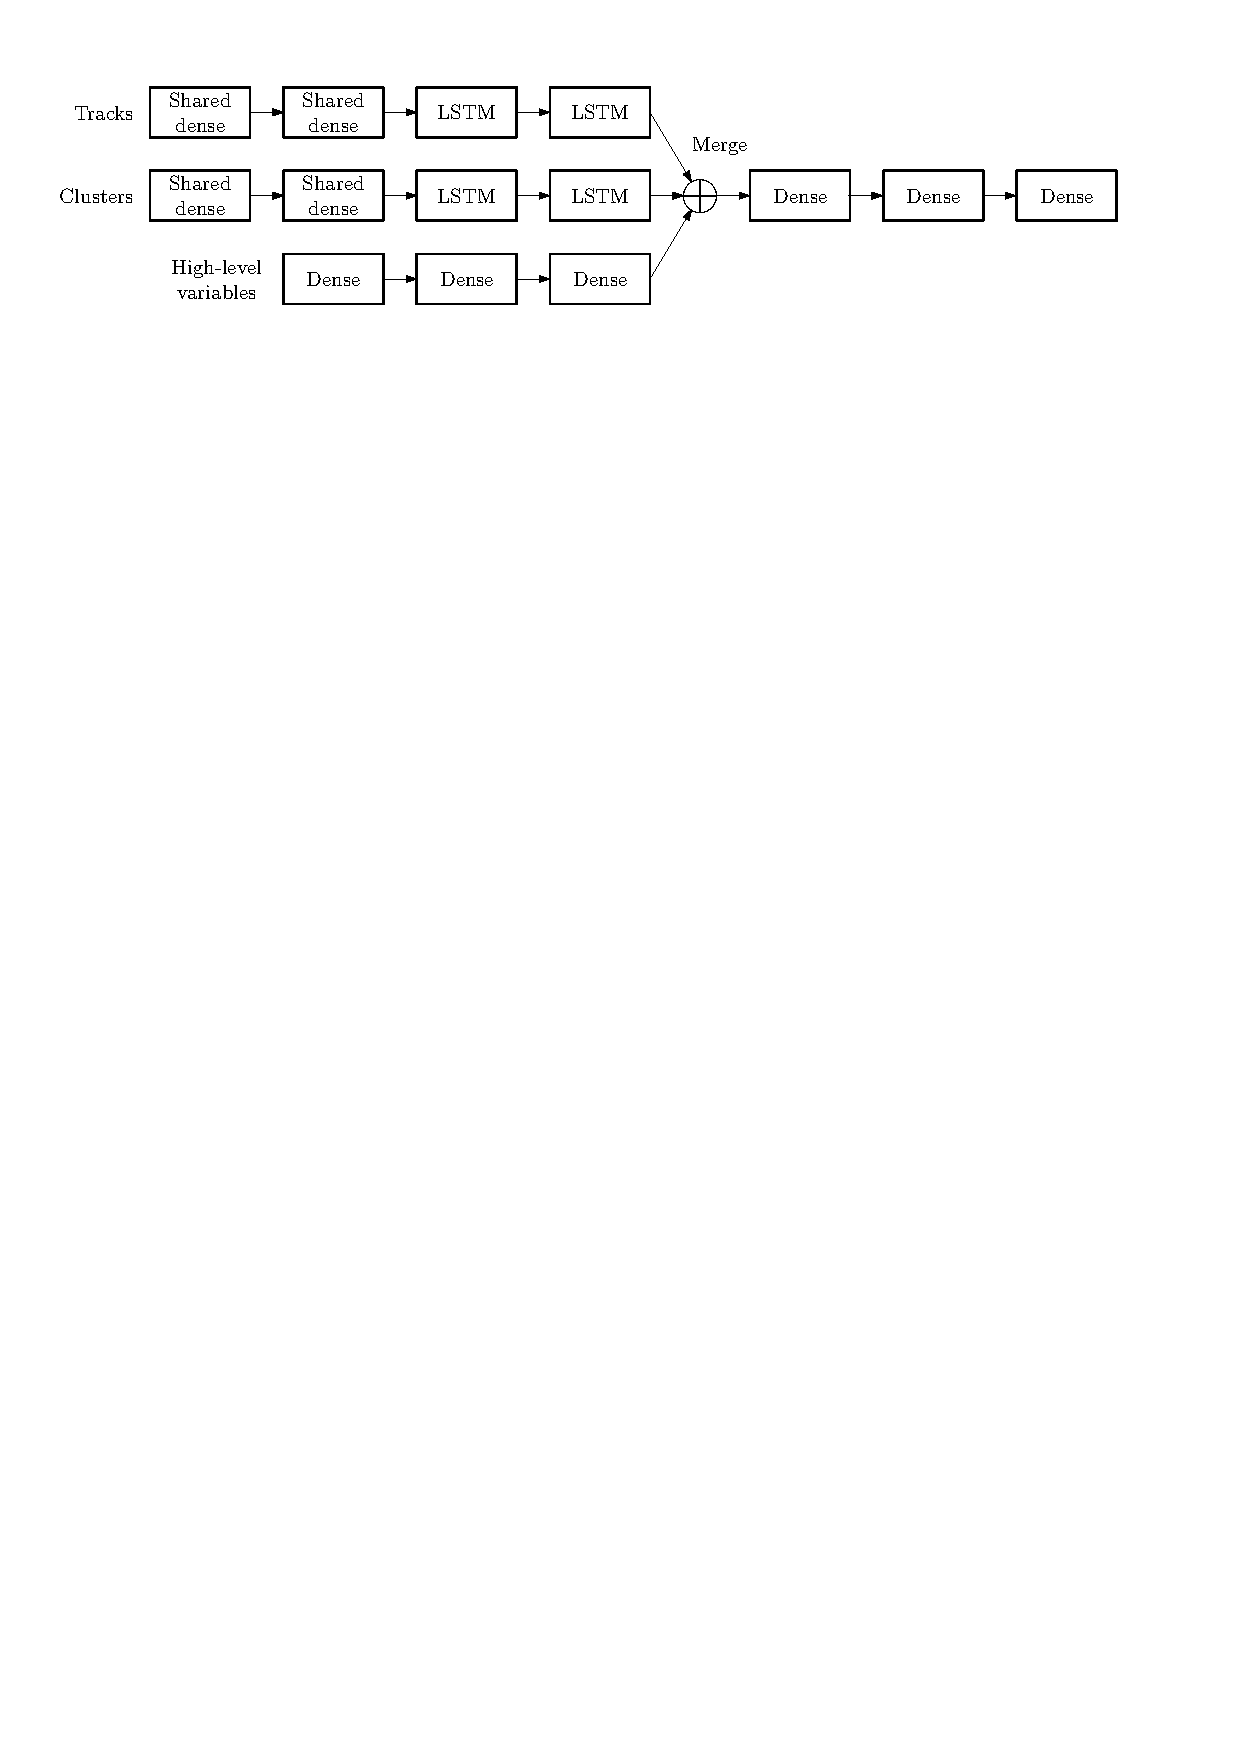
\includegraphics[width=0.95\textwidth]{tauid/pubnote/rnn_network_architecture}

  \caption{Network Architecture of the RNN \tauhad-identification
    algorithm \cite{ATL-PHYS-PUB-2019-033}}
  \label{fig:tauid_network_architecture}
\end{figure}

\subsection{Training and evaluation}

These samples are partitioned into a
training (\SI{40}{\percent}), validation (\SI{10}{\percent}), and
testing dataset (\SI{50}{\percent}).

Keras Tensorflow lwtnn \cite{lwtnn,keras,tensorflow2015-whitepaper,lstm}

Used in the software suite
\textsc{Athena}~\cite{ATL-SOFT-PUB-2021-001}.

\subsection{Working Point Definition}

\subsubsection{Calibration}

The efficiencies of the loose, medium, and tight working point for
\truetauhadvis were calibrated by the ATLAS collaboration using
$Z \to \tau_\mu \tauhad$ tag-and-probe showing agreement (within X
percent) between the predicted efficiency by simuation and the
efficiencies measured using collision data.


\section{Tau Identification Performance}
\label{sec:tauid_perf}

\begin{figure}[htbp]
  \centering

  % 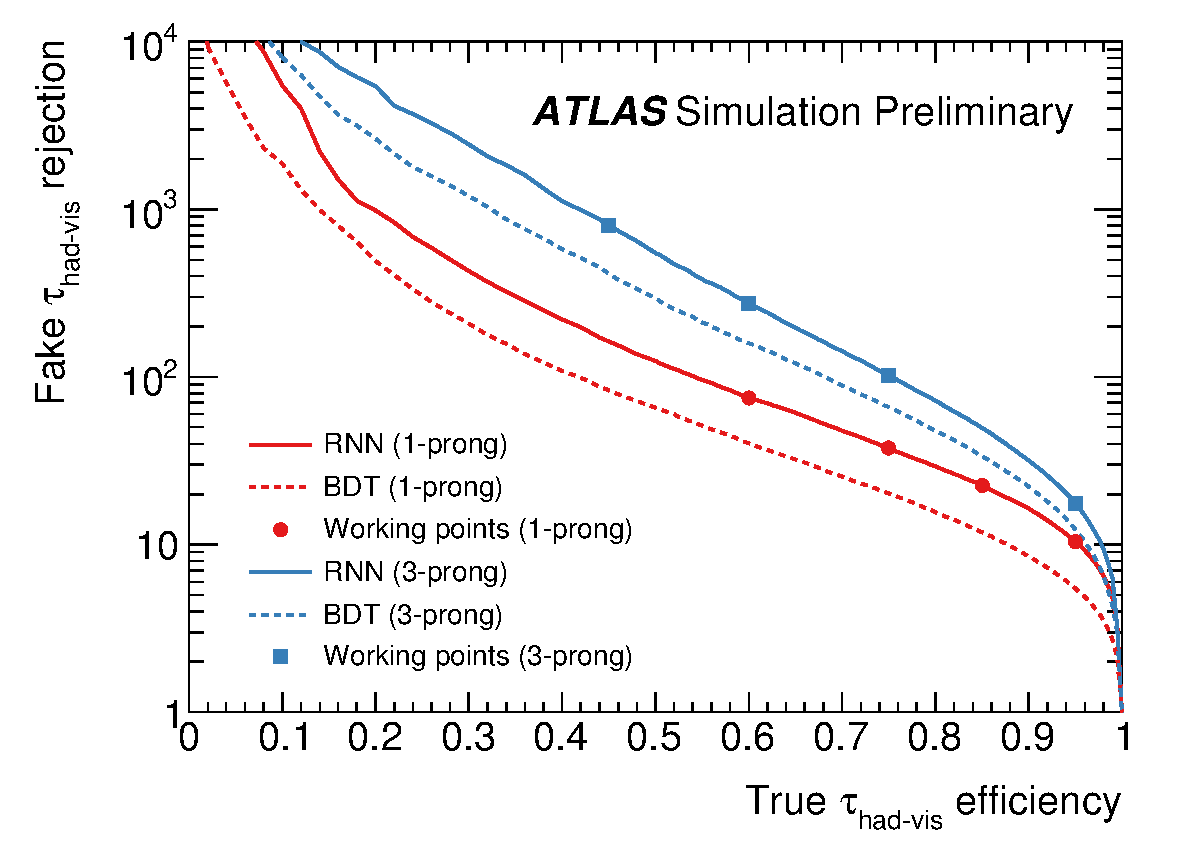
\includegraphics[width=0.55\textwidth]{tauid/pubnote/rnn_bdt_roc}
  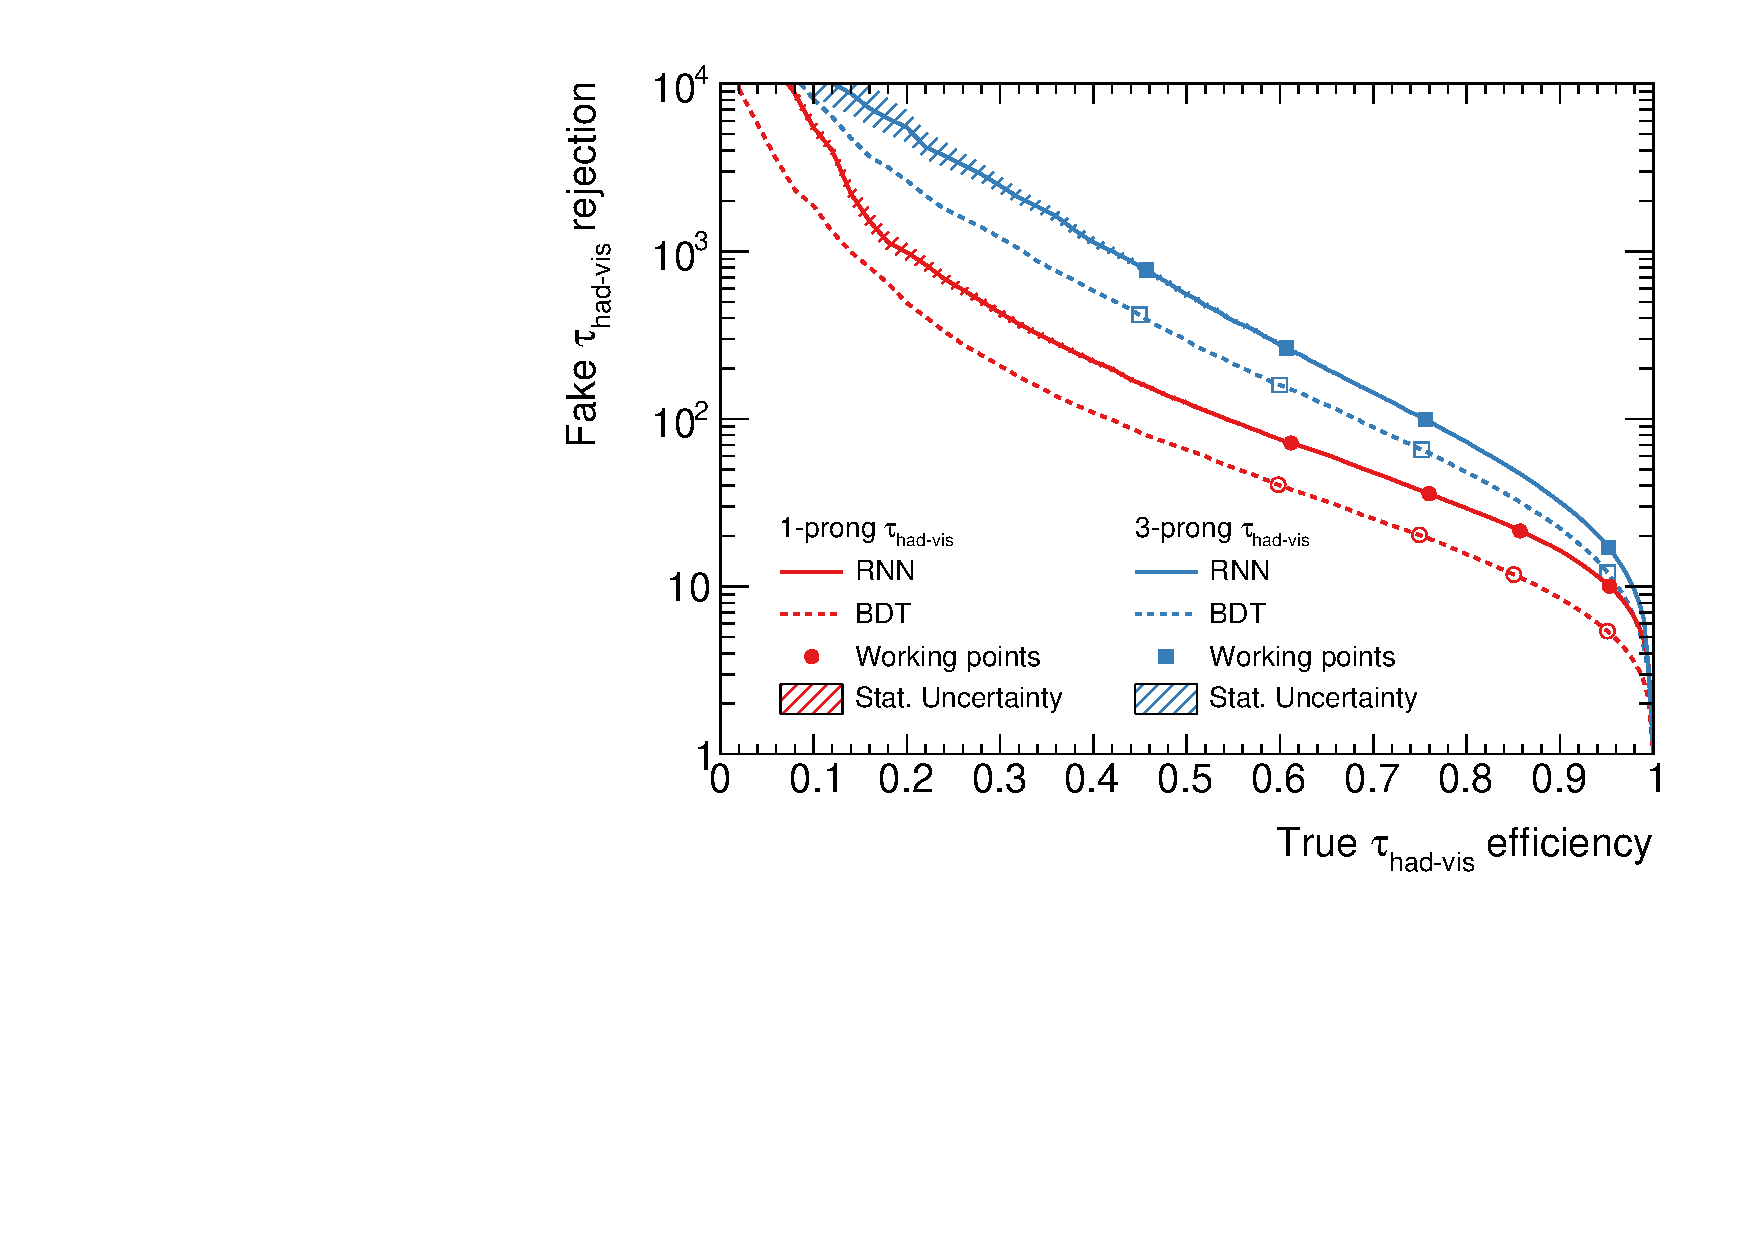
\includegraphics[width=0.55\textwidth]{tauid/roc_incl_witherrors}

  \caption{Receiver operating characteristic of the RNN
    \tauhad-identification algorithm \cite{ATL-PHYS-PUB-2019-033}}%
  \label{fig:tauid_rnn_bdt_roc_comparison}
\end{figure}


\begin{table}
  \centering

  \caption{List of defined working points with fixed true \tauhadvis
    selection efficiencies and the corresponding background rejection
    factors for misidentified \tauhadvis in dijet events for the BDT
    and RNN classifiers. Adapted from~\cite{ATL-PHYS-PUB-2019-033}.}%
  \label{tab:rnn_wps}

  \begin{tabular}{l
  cc
  @{\hskip 20pt}
  S[table-format=3.1]S[table-format=3.1]
  @{\hskip 20pt}
  S[table-format=3.1]S[table-format=3.1]}
  \toprule
  Working point & \multicolumn{2}{c@{\hskip 20pt}}{Signal efficiency} & \multicolumn{4}{c}{Background rejection} \\
  \cmidrule{4-7}
  &&& \multicolumn{2}{c@{\hskip 20pt}}{BDT} & \multicolumn{2}{c}{RNN} \\
                 & {1-prong} & {3-prong} & {1-prong} & {3-prong} & {1-prong} & {3-prong} \\
  \midrule
  Tight          & 60\,\%    & 45\,\%    & 40      & 420  & 72   & 770 \\
  Medium         & 75\,\%    & 60\,\%    & 20      & 160  & 36   & 260 \\
  Loose          & 85\,\%    & 75\,\%    & 12      & 66   & 21   & 99  \\
  Very loose     & 95\,\%    & 95\,\%    & 5.4     & 12   & 10   & 17  \\
  \bottomrule
\end{tabular}

% RNN tight 1P (rej): (71.96561246250148, 1.5303654439176062)
% RNN tight 1P (eff): (0.6117071909689276, 0.00024632688674175375)

% RNN tight 3P (rej): (773.933684779941, 39.28717816847519)
% RNN tight 3P (eff): (0.4566744467549334, 0.0003930521163405298)

% RNN medium 1P (rej): (35.82174458925124, 0.5877811653533531)
% RNN medium 1P (eff): (0.7597229941852967, 0.00028684295761911014)

% RNN medium 3P (rej): (264.41485204506034, 8.335133701736764)
% RNN medium 3P (eff): (0.6070290461673806, 0.00047597265519827683)

% RNN loose 1P (rej): (21.451007928217003, 0.2689671234302654)
% RNN loose 1P (eff): (0.8571601779651077, 0.00031300330970361357)

% RNN loose 3P (rej): (98.88497042998625, 1.8186512443248162)
% RNN loose 3P (eff): (0.756200706125848, 0.0005553554612403042)

% RNN veryloose 1P (rej): (10.059399296744843, 0.08444372648580398)
% RNN veryloose 1P (eff): (0.953066083106346, 0.0003384639200436791)

% RNN veryloose 3P (rej): (17.088578294479646, 0.13369860249913534)
% RNN veryloose 3P (eff): (0.9521385218793144, 0.0006570081893723098)

% BDT tight 1P (rej): (40.45967058185579, 0.7041781103272695)
% BDT tight 1P (eff): (0.5979792716851993, 0.00024250506003222104)

% BDT tight 3P (rej): (417.43136176200227, 16.77018703333453)
% BDT tight 3P (eff): (0.44928881105722246, 0.0003888705286576926)

% BDT medium 1P (rej): (20.35364225713967, 0.24775946939663773)
% BDT medium 1P (eff): (0.7493892746348453, 0.00028404624937242954)

% BDT medium 3P (rej): (159.3582135014997, 3.9403189472371616)
% BDT medium 3P (eff): (0.5996076427209064, 0.0004719599960117791)

% BDT loose 1P (rej): (11.788490308526693, 0.10777438892574735)
% BDT loose 1P (eff): (0.850531538104052, 0.000311232976426111)

% BDT loose 3P (rej): (65.58988709376405, 0.978622556721974)
% BDT loose 3P (eff): (0.7517812018543497, 0.0005530325740489808)

% BDT veryloose 1P (rej): (5.423518802654415, 0.03531494188085259)
% BDT veryloose 1P (eff): (0.9508788348923811, 0.00033788569007909387)

% BDT veryloose 3P (rej): (12.100080401977765, 0.08023605419699714)
% BDT veryloose 3P (eff): (0.9511017578180401, 0.0006564758961708566)

%%% Local Variables:
%%% mode: latex
%%% TeX-master: "../phd_thesis"
%%% End:

\end{table}


\begin{figure}[htbp]

  \begin{subfigure}{0.498\textwidth}
    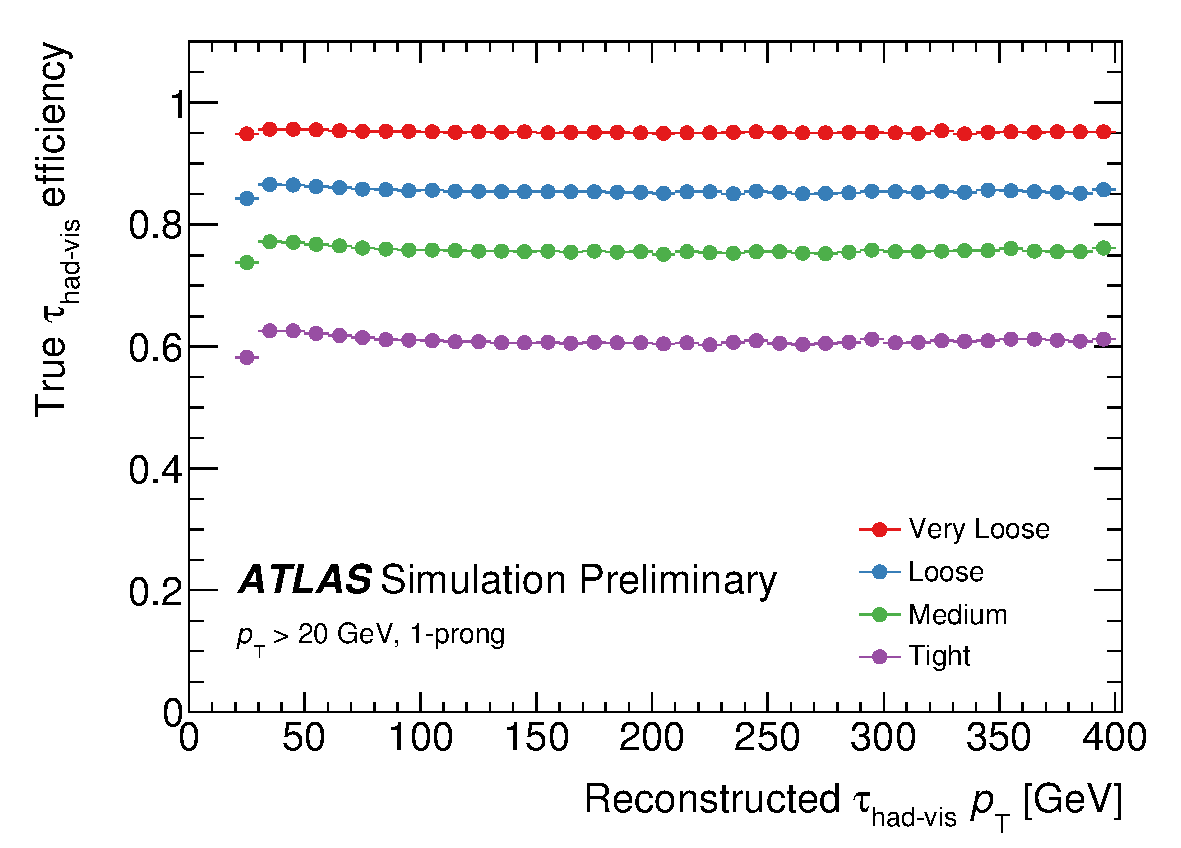
\includegraphics[width=\textwidth]{tauid/pubnote/eff_vs_pt_1p}
    \subcaption{}
  \end{subfigure}\hfill%
  \begin{subfigure}{0.498\textwidth}
    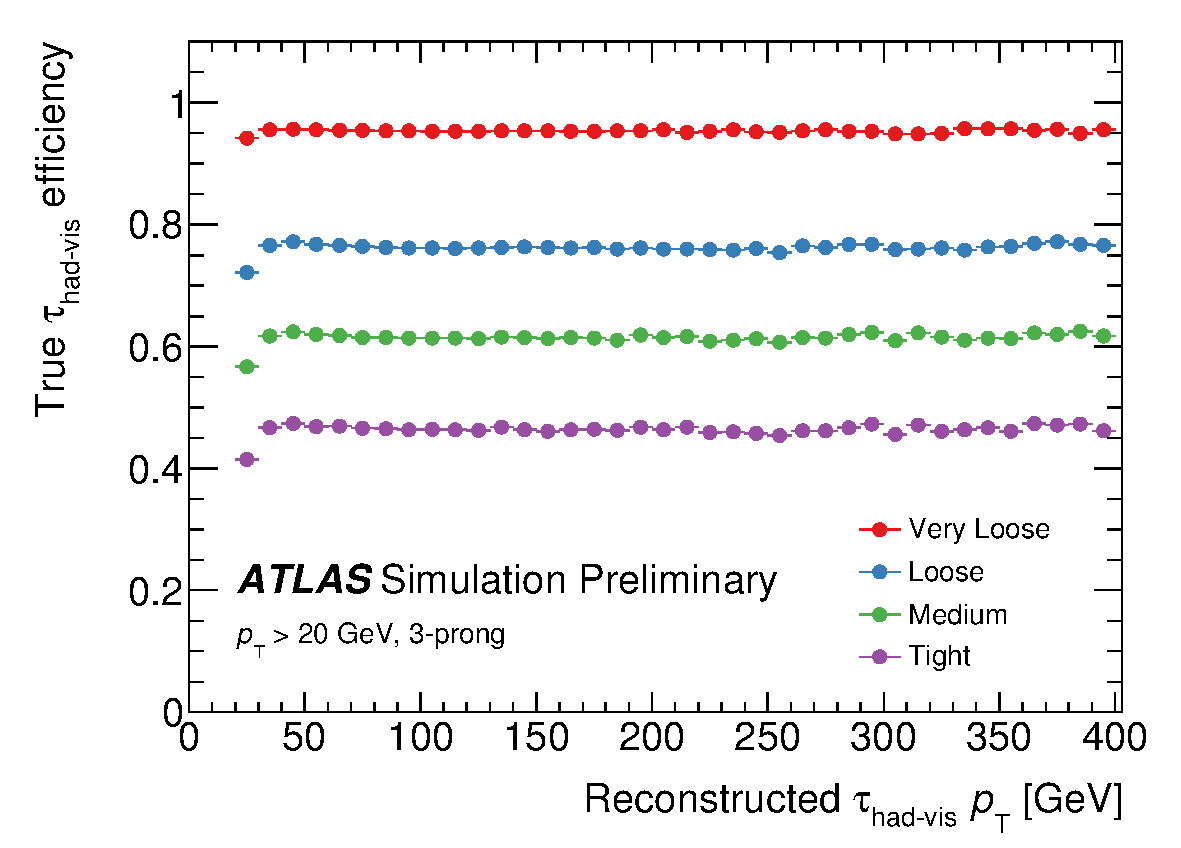
\includegraphics[width=\textwidth]{tauid/pubnote/eff_vs_pt_3p}
    \subcaption{}
  \end{subfigure}

  \begin{subfigure}{0.498\textwidth}
    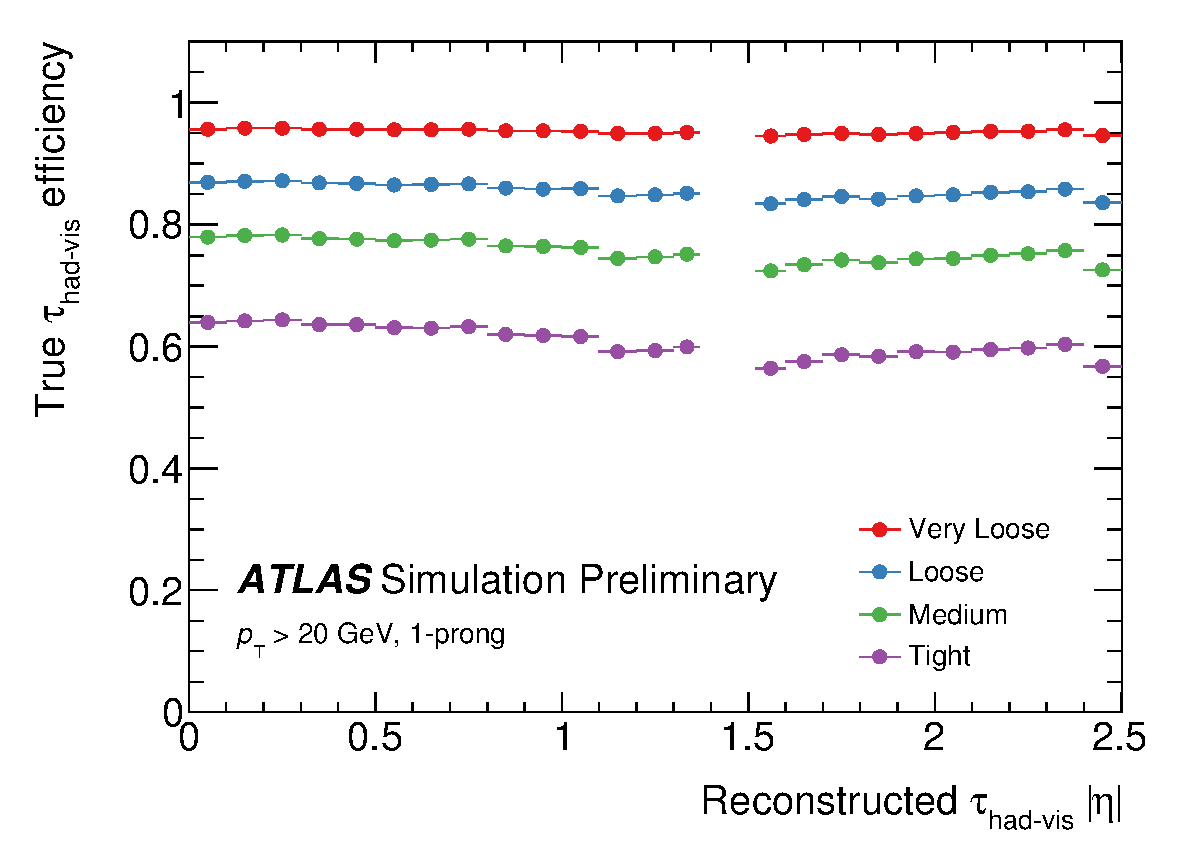
\includegraphics[width=\textwidth]{tauid/pubnote/eff_vs_eta_1p}
    \subcaption{}
  \end{subfigure}\hfill%
  \begin{subfigure}{0.498\textwidth}
    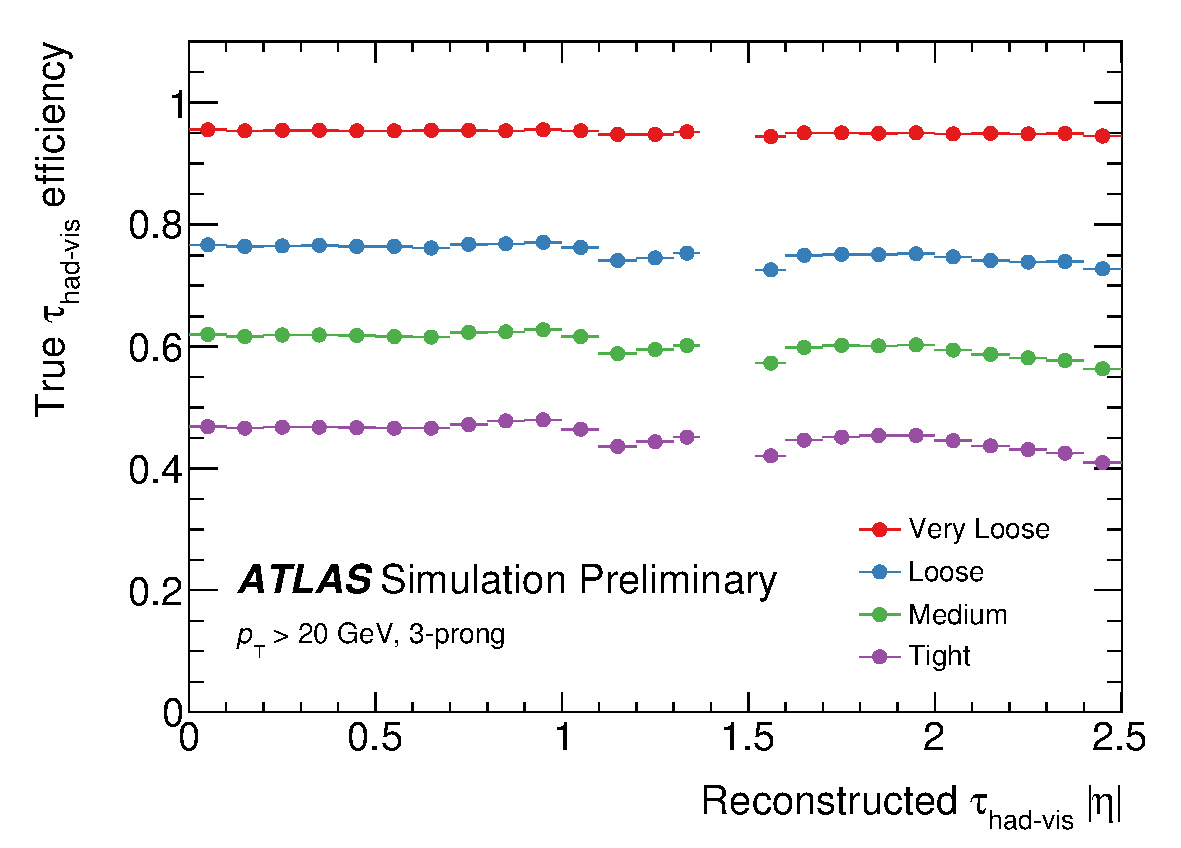
\includegraphics[width=\textwidth]{tauid/pubnote/eff_vs_eta_3p}
    \subcaption{}
  \end{subfigure}

  \begin{subfigure}{0.498\textwidth}
    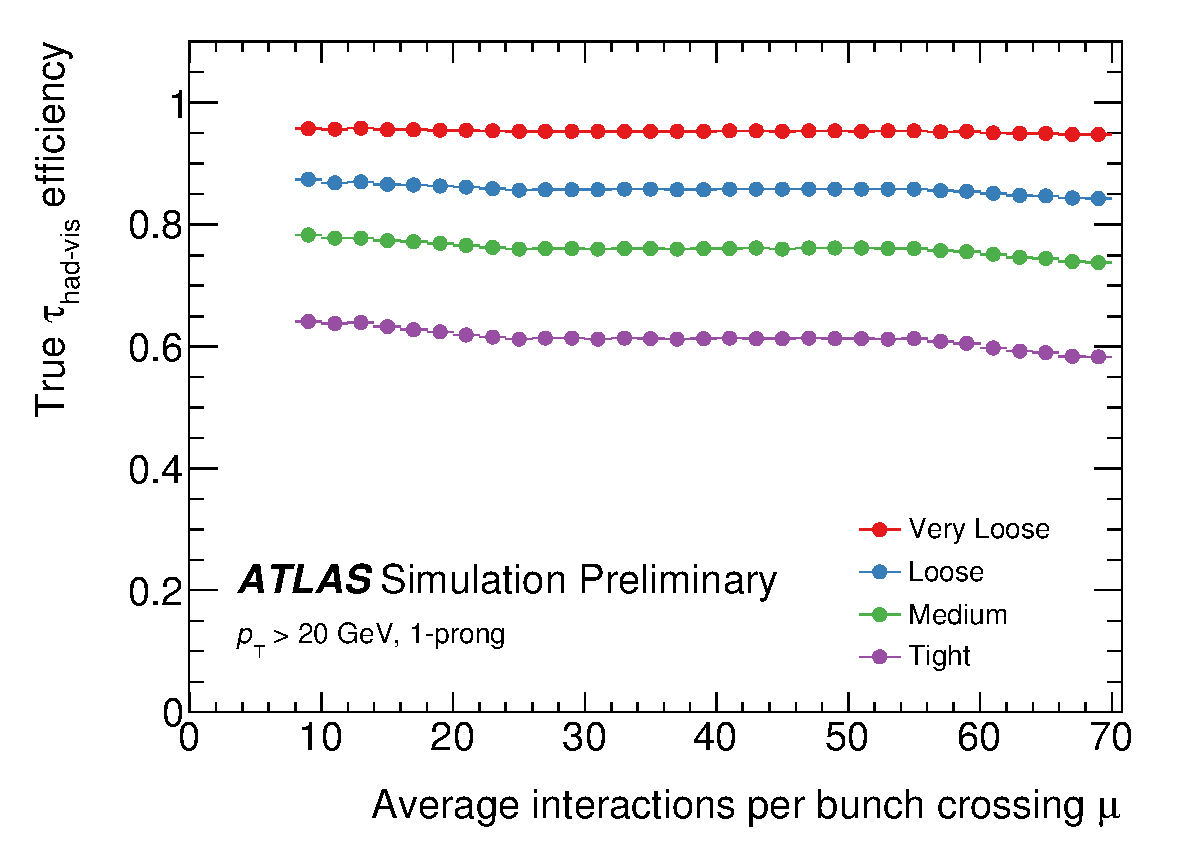
\includegraphics[width=\textwidth]{tauid/pubnote/eff_vs_mu_1p}
    \subcaption{}
  \end{subfigure}\hfill%
  \begin{subfigure}{0.498\textwidth}
    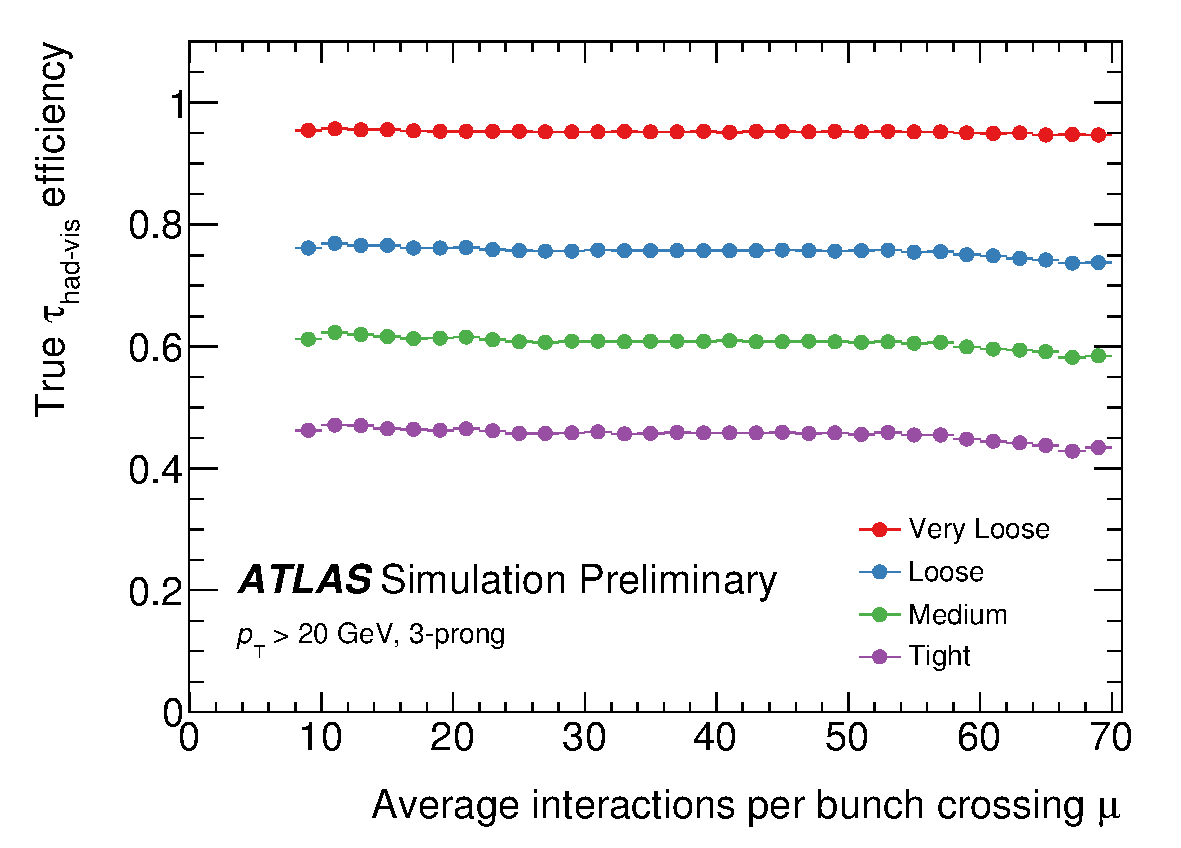
\includegraphics[width=\textwidth]{tauid/pubnote/eff_vs_mu_3p}
    \subcaption{}
  \end{subfigure}

  \caption{Eff. Figures are taken from
    Ref.~\cite{ATL-PHYS-PUB-2019-033}.}
  \label{fig:tauid_truetau_eff}
\end{figure}





\subsection{Use at the HLT?}

\cite{ATL-DAQ-PUB-2019-001}


\section{Conclusion and Outlook}
\label{sec:tauid_conclusion}


To be replaced by ``deep sets'' (permutation invariance). Based on the
same idea and same expected performance but significantly improved
training and prediction time.

%%% Local Variables:
%%% mode: latex
%%% TeX-master: "../../phd_thesis"
%%% End:
